% =========================================================================
%        LaTeX Template for PhD Thesis
% =========================================================================

%\RequirePackage[l2tabu, orthodox]{nag} % display more warnings

\documentclass{sokendai_thesis} % for final version
%\documentclass[todo]{sokendai_thesis} % print todo notes (generated by this command: \mytodo[inline]{this is just a todo note})


% =====================================================
%  User-defined Commands
% =====================================================

\newcommand{\Order}{\mathit{O}} % for computational complexity


% =====================================================
%  Thesis Info
% =====================================================

\title{A Study on Portable Load Balancer for Container Clusters}
\author{Kimitoshi Takahashi}
\date{September 2019}
\crest{Figs/sokendai-logomark.png} % comment out if you don't have a crest.
%\keywords{Latex Template, Sokendai, PhD Thesis} % for PDF meta-info

\usepackage{xcolor}
\definecolor{mygray}{rgb}{0.95,0.99,0.99}

\usepackage[final]{changes}

% =====================================================
%  Others
% =====================================================

% Typeset only specified chapters
%\includeonly{Manuscript/Introduction/introduction}


% =====================================================
%  Front Matter
% =====================================================

\begin{document}

\frontmatter
\maketitle

% \listoftodos

\chapter*{Acknowledgments}

[Filled in later]
%I would like to thank ...

\mytodo[inline]{Write Acknowledgments.}




\chapter*{Abstract}

Linux containers have become very popular these days due to their lightweight nature and portability. 
Numerous web services are now deployed as clusters of containers. 
Kubernetes is a popular container management system that enables users to deploy such web services easily, and hence, 
it facilitates web service migration to the other side of the world.
However, since Kubernetes relies on external load balancers provided by cloud providers, 
it is difficult to use in environments where there are no supported load balancers.
This is particularly true for on-premise data centers, or for all but the largest cloud providers.
In this paper, we proposed a portable load balancer that was usable in any environment, and hence facilitated web services migration.
We implemented a containerized software load balancer that is run by Kubernetes as a part of container cluster, 
using Linux kernel's Internet Protocol Virtual Server(IPVS).
Then we compared the performance of our proposed load balancer with existing iptables Destination Network Address 
Translation (DNAT) and the Nginx load balancers.
During our experiments, we also clarified the importance of two network conditions to derive the best performance: 
the first was the choice of the overlay network operation mode, and the second was distributing packet processing to multiple cores.
The results indicated that our proposed IPVS load balancer improved portability of web services without sacrificing the performance.


Linux container technology and clusters of the containers are expected to make web services consisting of multiple web servers and a load balancer portable, and thus realize easy migration of web services across the different cloud providers and on-premise datacenters.
This prevents service to be locked-in a single cloud provider or a single location and enables users to meet their business needs, e.g., preparing for a natural disaster.
However existing container management systems lack the generic implementation to route the traffic from the internet into the web service consisting of container clusters.
For example, Kubernetes, which is one of the most popular container management systems, is heavily dependent on cloud load balancers. If users use unsupported cloud providers or on-premise datacenters, it is up to users to route the traffic into their cluster while keeping the redundancy and scalability.
This means that users could easily be locked-in the major cloud providers including GCP, AWS, and Azure.
In this paper, we propose an architecture for a group of containerized load balancers with ECMP redundancy.
We containerize Linux ipvs and exabgp, and then implement an experimental system using standard Linux boxes and open source software.
We also reveal that our proposed system properly route the traffics with redundancy.
Our proposed load balancers are usable even if the infrastructure does not have supported load balancers by Kubernetes and thus free users from lock-ins.



\tableofcontents
\listoffigures
\listoftables
%% List of algorithms
%\listofalgorithms \addcontentsline{toc}{chapter}{List of Algorithms}

% =====================================================
%  Main Matter
% =====================================================

\mainmatter

%-----------------------------------------------------------
%
\graphicspath{{Manuscript/}}

\chapter{Introduction}\label{chapter:introduction}

Recently, launching web services on cloud computing infrastructure is getting more popular.
Launching web services on the cloud is easier than launching them on on-premise data centers.
A web service on the cloud becomes scalable, which means it can accommodate a large amount of traffic from the Internet by increasing the number of web servers, on demand.
To distribute high volume traffic from the Internet to thousands of web servers load balancers are often used.
Major cloud providers have developed software load balancers\cite{eisenbud2016maglev,patel2013ananta} as part of their infrastructures, which they claim to have a high-performance level and scalability.
In the case of on-premise data centers, one can use proprietary hardware load balancers.
The actual implementation and the performance level of those existing load balancers are very different.

As for another issue regarding web services,
there are also needs to use multiple of cloud providers or on-premise data centers seamlessly, which spread across the world, to prepare for the disaster, to lower the cost or to comply with the legal requirement.
Linux container technology\cite{menage2007adding} facilitates these usages by providing container cluster management system as a middleware,
where one can deploy a web service that consists of a cluster of containers without modification even on different infrastructures.
However, in reality, it is difficult to do so, because existing load balancers are very different and are not included in the container cluster management system.
Therefore, users should always manually adjust their web services to the infrastructure.

In short, there exist several software load balancers that are specific to cloud vendors and on-premise data centers.
The differences among them are the major obstacles to provide uniform container cluster platform, which is necessary to realize web service migration across the different cloud providers and on-premise data centers.

To address this problem, we propose a portable and scalable software load balancer that can be used in any environment including cloud providers and in on-premise data centers.
We can include this load balancer as a part of a container cluster management system, e.g., Kubernetes\cite{K8s2017}, which acts as a common middleware on which web services run.
Users now do not need manual adjustment of their services to the infrastructures.
We will implement the proposed software load balancer using following technologies;
1) To make the load balancer usable in any environment, we containerize ipvs\cite{Zhang2000} using Linux container technology\cite{menage2007adding}.
2) To make the load balancer scalable, we make it capable of being run in parallel using Equal Cost Multi-Path(ECMP) technique\cite{al2008scalable}.
In order to make the load balancer's performance level to meet the need for 10Gbps network speed, a software load balancer that better performs than ipvs is required.
We also implement the novel load balancer using eXpress Data Plane(XDP) technology\cite{bertin2017xdp}.

The outcome of our study will benefit users who want to deploy their web services on any cloud provider where no scalable load balancer is provided, to achieve high scalability.
Moreover, the result of our study will potentially benefit users who want to use a group of different cloud providers and on-premise data centers across the globe, as if it were a single computer on which their web services run.

The rest of the paper is organized as follows.
Section \ref{Related Work} highlights work that deals specifically with container cluster migration, 
software load balancer containerization, and load balancer related tools within the context of the container technology. 
Section \ref{Architecture} will explain existing architecture problems and propose our solutions.
In Section \ref{Experiments}, experimental results for containerized ipvs are discussed,  
which is followed by a summary of our work in Section~\ref{Conclusions}.






\chapter{Background}\label{chapter:background}
\section{Kuberenetes}

\begin{figure}
\includegraphics[width=\columnwidth]{Figs/K8sConventional}
\caption{Conventional architecture of a Kubernetes cluster.}
\label{fig:K8sConventional}
\end{figure}

Problems commonly occur when the Kubernetes container management system is used outside of recommended cloud providers(such as GCP or AWS).
Figure~\ref{fig:K8sConventional} shows an exemplified Kubernetes cluster.
A Kubernetes cluster typically consists of a master and nodes. They can be physical servers or VMs.
On the master, daemons that control the Kubernetes cluster are typically deployed. 
These daemons include, apiserver, scheduler, controller-manager and etcd. 
On the nodes, the kubelet daemon will run {\it pods}, depending the PodSpec information obtained from the apiserver on the master.
A {\em pod} is a group of containers that share same net name space and cgroups, 
and is the basic execution unit in a Kubernetes cluster.

When a service is created, the master will schedule where to run {\em pods} and kubelets on the nodes will launch them accordingly.
At the same time, the masters will send out requests to cloud provider API endpoints, asking them to set up external cloud load balancers.
The proxy daemon on the nodes will also setup iptables DNAT\cite{MartinA.Brown2017} rules. 
The Internet traffic will then be evenly distributed by the cloud load balancer to nodes, 
after which it will be distributed again by the DNAT rules on the nodes to the designated {\em pods}. 
The returning packets will follow the exact same route as the incoming ones.

This architecture has the followings problems: 
1) Having cloud load balancers whose APIs are supported by the Kubernetes daemons is a prerequisite.
There are numerous load balancers which is not supported by the Kubernetes.
These include the bare metal load balancers for on-premise data centers.  
In such cases, users are required to set up the routing manually depending on the infrastructure.
The traffic would be routed to a node then distributed by the DNAT rules on the node to the designated {\em pods}.
However, this approach significantly degrades the portability of container clusters.

2) Distributing the traffic twice, first on the external load balancers and second on each node, 
complicates the administration of packet routing. 
Imagine a situation in which the DNAT table on one of the nodes malfunctions.
In such a case, only occasional timeouts would be observed, which would make it very difficult to find out which node was malfunctioning.   

In short, 1) Kubernetes can be used only in limited environments where the external load balancers are supported, 
and 2) the routes incoming traffic follow are very complex.

In order to address these problems, we propose a containerized software load balancer 
that is deployable in any environment even if there are no external load balancers.

\section{Overlay Network}\label{sec:overlay_network}

In order to discuss load balancer redundancy, the knowledge of the overlay network is essential.
We briefly explain an abstract concept of overlay network that is common to existing overlay network including flannel\cite{coreos_2018} and calico\cite{project_calico}.

\begin{figure}[tb]
\begin{center}
\includegraphics[width=\columnwidth]{Figs/overlay.png}
\end{center}
\caption{
  The network architecture of an exemplified container cluster system. %\\ %\par
  A load balancer(lb) pod(the white box with "lb") and web pods are running on nodes(the blue boxes).
  The traffic from the internet are forwarded to the lb pod by the upstream router using the node network,
  and the distributed to web pods using the overlay network.
}
\label{fig:overlay}
\end{figure}

Fig.~\ref{fig:overlay} shows schematic diagram of network architecture of a container cluster system. 
Suppose we have a physical network(node network) with IP address range of 10.0.0.0/16 and an overlay network with IP address range of 172.16.0.0/16.
The node network is the network for nodes to communicate with each other.
The overlay network is the network setups for containers to communicate with each other.
An overlay network typically consists of appropriate routing tables on nodes, and optionally of tunneling setup using ipip or vxlan.
The upstream router usually belongs to the node network.
When a container in the Fig.~\ref{fig:overlay} communicates with any of the nodes, it can use its IP address in 172.16.0.0/16 IP range as a source IP, since every node has proper routing table for the overlay network.
When a container communicates with the upstream router that does not have routing information regarding the overlay network, the source IP address must be translated by Source Network Address Translation(SNAT) rules on the node the container resides.

The SNAT caused a problem when we tried to co-host multiple load balancer containers for different services on a single node, and let them connect the upstream router directly.
This was due to the fact that the BGP agent used in our experiment only used the source IP address of the connection to distinguish the BGP peer.
The agent behaved as though different BGP connections from different containers belonged to a single BGP session because the source IP addresses were identical due to the SNAT.

\subsection{Flannel}
\paragraph{\bf host-gw}
\paragraph{\bf vxlan}
\paragraph{\bf udp}

\subsection{Calico}
\paragraph{\bf no-tunnel}
\paragraph{\bf ipip}

\section{Multicore Packet Proccessing}
\subsection{rss}
\subsection{rps}
\subsection{Others}
\paragraph{rfs}
\paragraph{xps}
\paragraph{xfs}

\section{Other parameters}
\subsection{tcp congestion mode}

\section{Cloud Load Balancers}
\subsection{Maglev}
\subsection{Ananta}
\subsection{GCP Load Balancer}
GCP experimental data.


\chapter{Architecture and Implementation}\label{chapter:Architecture and Implementation}
This chapter provides discussion of load balancer architecture suitable for container clusters.
First the author discusses problems of conventions architecture in Section~\ref{Problem of Conventional Architecture}.
Then the author proposes a portable software load balancer in container in Section~\ref{Load balancer in container}
After that the author discusses redundancy architecture using ECMP in Section~\ref{Redundancy with ECMP}. 

This chapter also presents implementation of the proof of the concept system for the proposed load balancer architecture in detail.
First overall architecure is explained in Section~\ref{sec:poc}.
Then ipvs containerization is explained in detail in Section~\ref{sec:ipvs}.
Finally implementation of BGP software container is explained in Section~\ref{sec:bgp}.

\section{Architecture}

In this section the author discusses the architecture of a portable load balancer for container clusters.

\subsection{Problem of Conventional Architecture}\label{Problem of Conventional Architecture}

\begin{figure}[tb]

  \begin{subfigure}[t]{\columnwidth}
    \centering
    \includegraphics[width=0.8\columnwidth]{Figs/K8sConventional}
    \caption{Kubernetes in cloud infrastructures}
    \label{fig:K8sConventional}
  \end{subfigure}

  \par\bigskip
  \par\bigskip

  \begin{subfigure}[t]{\columnwidth}
    \centering
    \includegraphics[width=0.8\columnwidth]{Figs/K8sConventional_bm}
    \caption{Kubernetes in on-premise data centers}
    \label{fig:K8sConventional_bm}
  \end{subfigure}

  \caption{Conventional architecture of Kubernetes clusters in cloud infrastructure and on-premise data center}
  
  \centering
  \begin{minipage}{0.9\columnwidth}
    In supported infrastructures, e.g., major cloud providers, Kubernetes automatically set up a route to an IP address for a service(the author calls this address, service IP), when web service providers a launch container cluster.
    In unsupported infrastructures, e.g., on-premise data centers, they have to manually set up the route.
  \end{minipage}

%  \label{fig:exabgp}
\end{figure}

The problem of Kubernetes is its partial support for the ingress traffic routing.
Figure~\ref{fig:K8sConventional} shows an exemplified Kubernetes cluster.
A Kubernetes cluster typically consists of a master and nodes. They can be physical servers or VMs.
On the master, daemons that control the Kubernetes cluster are typically deployed. 
These daemons include, apiserver, scheduler, controller-manager and etcd. 
On the nodes, kubelet and proxy are deployed.
The kubelet daemon will run {\it pods}, depending on the PodSpec (pod specification) information obtained from the apiserver on the master.
The proxy daemon will set up iptables DNAT rules that function as the internal load balancer.
A {\em pod} is a group of containers that share the same network namespace and cgroup,
and is the basic execution unit in a Kubernetes cluster.

When a service is created, the master schedules where to run {\em pods} and kubelets on the nodes launch them accordingly.
At the same time, the master sends out requests to cloud provider's API endpoints, asking them to set up external cloud load balancers that distribute ingress traffic to every node in the Kubernetes cluster.
The proxy daemon on the nodes also setup iptables DNAT\cite{MartinA.Brown2017} rules. 
The Ingress traffic will then be evenly distributed by the cloud load balancer to nodes, 
after which it will be distributed again by the DNAT rules on the nodes to the designated {\em pods}. 
The returning packets follows the exact same route as the incoming ones.

This architecture has the followings problems: 
1) There must exist cloud load balancers whose APIs are supported by the Kubernetes daemons.
There are numerous load balancers which is not supported by the Kubernetes.
These include the bare metal load balancers for on-premise data centers.
2) Distributing the traffic twice, first on the external load balancers and second on each node, complicates the administration of packet routing. 
Imagine a situation in which the DNAT table on one of the nodes malfunctions.
In such a case, only occasional timeouts would be observed, and hence it would be very difficult to find out which node is malfunctioning.   

Regarding the first problem, if there is no load balancer that is not supported by Kubernetes, users must manually set up the static route on the upstream router, every time they launch the web application clusters, as is shown in Figure~\ref{fig:K8sConventional_bm}.
The traffic would be routed to a node then distributed by the DNAT rules on the node to the designated {\em pods}.
However, in the cases where the upstream router is administered by different organizations, users are always required to negotiate with them about adding a route to their new application cluster.
Therefore this approach significantly degrades the portability of container clusters.
Furthermore, a static route usually lacks redundancy and scalability.

In short, 1) while Kubernetes is effective in major cloud providers, it fails to provide portability for container clusters in environments where there is no supported load balancer, and 2) the routes incoming traffic follow are very complex.
In order to address these problems, the author proposes a containerized software load balancer 
that is deployable in any environment even if there are no external load balancers.

\FloatBarrier

\subsection{Load balancer in container}\label{Load balancer in container}

The author proposes a load balancer architecture, where a cluster of load balancers are deployed as containers.
Figure~\ref{fig:K8sProposed} shows the proposed load balancer architecture for Kubernetes,
which has the following characteristics;
1) Each load balancer itself is run as a {\em pod} by Kubernetes. 
2) Load balancing tables are dynamically updated based on information about running {\em pods}.
3) There exist multiple load balancers for redundancy and scalability.
4) The routing table in the upstream router are updated dynamically using standard network protocol.

\begin{figure}[h]
  \begin{center}
  \includegraphics[width=0.8\columnwidth]{Figs/K8sProposed}
  \caption{Kubernetes cluster with proposed load balancer.}
  \label{fig:K8sProposed}
  \begin{minipage}{0.9\columnwidth}
  Each load balancer itself is run as a {\em pod} by Kubernetes. 
  Load balancing tables are dynamically updated based on information about running {\em pods}.
  There exist multiple load balancers for redundancy and scalability.
  The routing table in the upstream router are updated dynamically using standard network protocol.
  \end{minipage}
  \end{center}
\end{figure}

The proposed load balancer can resolve the conventional architecture problems.
Since the load balancer itself is containerized, the load balancer can run in any environment including on-premise data centers,
even without external load balancers that is supported by Kubernetes.
The incoming traffic is directly distributed to designated {\em pods} by the load balancer.
It makes the administration, e.g. finding malfunctions, easier.

Furthermore, the proposed load balancer has other benefits.
Since a software load balancer in a container can run on any Linux system, it can share the server pool with web containers.
Users can utilize existing servers rather than buying dedicated hardware.

Because a cluster of load balancer containers is controlled by Kubernetes, it becomes redundant and scalable.
Kubernetes always tries to maintain the number of load balancer containers at the number specified by the user.
If a single container fails, Kubernetes schedule and launch another one on a different node, which provides the resilience to failures.
When there is a huge spike in the traffic, it can quickly scale the size of the cluster depending on the demand.

The routes to the load balancers are automatically updated through the standard protocol, BGP.
Therefore users do not need to manually add the route every time new load balancer container is launched, as is the case in the conventional architecture.

\FloatBarrier

\subsection{Redundancy with ECMP}\label{Redundancy with ECMP}

\begin{figure}[tb]
  \centering
  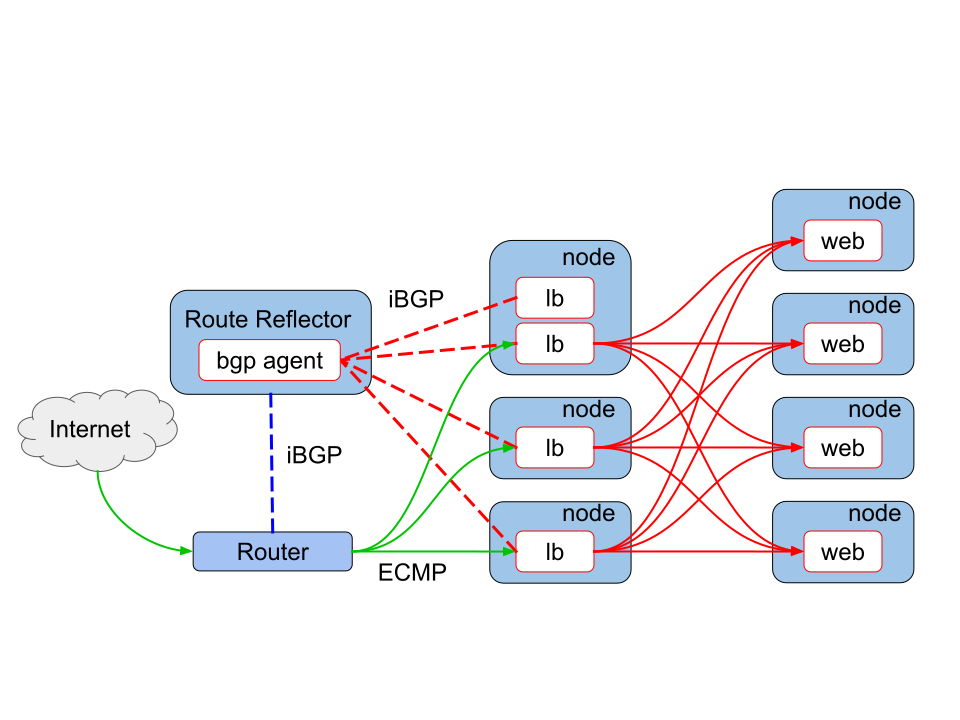
\includegraphics[width=0.8\columnwidth]{Figs/ecmp.png}
\caption{The proposed architecture of load balancer redundancy with ECMP}

\vspace{1mm}

\begin{minipage}{0.9\columnwidth}
  The traffic from the internet is distributed by the upstream router to multiple of lb pods using hash-based ECMP(the solid green line) and then distributed by the lb pods to web pods using Linux kernel's ipvs(the solid red line).
  The route to an IP address for a service(the author calls this address, service IP) is advertised to the route reflector(the dotted red line) and then advertised to the upstream router(the blue dotted line) using iBGP.
  For the green lines, a service IP address is used. The red lines use the IP addresses of the overlay network. The blue line uses the IP addresses of the node network.
\end{minipage}

\label{fig:ecmp}
\end{figure}

While containerizing ipvs makes it runnable in any environment, it is essential to discuss how to route the traffic to the ipvs container.
The author proposes redundant architecture using ECMP with BGP for load balancer containers usable especially in on-premise data centers.

Fig.~\ref{fig:ecmp} shows a schematic diagram to explain redundancy architecture with ECMP for the proposed load balancer.
%
The ECMP is a functionality a router supports, where the router has multiple next hops with equal priority(cost) to a destination.
And the router generally distributes the traffic to the multiple next hops depending on the hash of five-tuples(source IP, destination IP, source port, destination port, protocol) of the flow.
The multiple next hops and their cost are often populated using the BGP protocol.
%
The notable benefit of the ECMP setup is its scalability.
All the load balancers that claims as the next hop is active, i.e., all of them are utilized to increase the performance level.
Since the traffic from the internet is distributed by the upstream router, the overall throughput is limited by performance levels of the router after all.
However, in practice, there are a lot of cases where this architecture is beneficial.
For example, if a software load balancer is capable of handling 1 Gbps equivalent of traffic and the upstream router is capable of handling 10 Gbps, it still is worthwhile launching 10 of the software load balancer containers to fill up maximum throughput of the upstream router.

%
In the proposed redundant architecture, there exists a node with the knowledge of the overlay network as a route reflector
A route reflector is a network component for BGP to reduce the number of peerings by aggregating the routing information\cite{rfc4456}.
In the proposed architecture the author uses it as a delegater for load balancer containers towards the upstream router.

The route reflector exists for a practical reason, i.e, to deal with the complexity due to the overlay network.
Since the upstream router normally has no knowledge of the overlay network and IP addresses used inside the Kubernetes clusters, a container must rely on SNAT on the node to communicate with the router.
The SNAT caused a problem when the author tried a set up without the route reflector, to co-host multiple load balancer containers for different services on a single node.
Because of the SNAT, the source IP addresses of multiple connections were translated into a single IP address possessed by the node.
The BGP agent on the router was confused by these connections and could not properly set up ECMP routes for separate services.
This was due to the fact that the BGP agent used in the experiment used only the source IP address of the connection to distinguish the BGP peer.

In addition to that, the route reflector brings another benefit.
The upstream router does not need to accept BGP sessions from containers with random IP addresses, but only from the route reflector with well known fixed IP address.
This is preferable in terms of security especially when a different organization administers the upstream router.

By using the route reflector, we can have the following benefits.
1) Each node can accommodate multiple load balancer containers. This was not possible when we tried to directly connect load balancers and the router through SNAT.
2) The router does not need to allow peering connections from random IP addresses that may be used by load balancer containers. Now, the router only need to have the reflector information as the BGP peer definition.

Since a standard Linux box is used for the route reflector, it can be configured as the user likes;
a) It can be configured to belong to the overlay network so that multiple BGP sessions from a single node can be established.
b) A BGP agent that supports dynamic neighbor (or dynamic peer) can be used, where one only needs to define the IP range as a peer group and does away with specifying every possible IP that load balancers may use.
Although not shown in the Fig.~\ref{fig:ecmp}, it is possible to have another route reflector for redundancy purpose.

\FloatBarrier



\section{Implementation}

In this section the author discusses the implementation of the experimental system to prove the concept of our proposed load balancers with ECMP redundancy in detail.

\subsection{Experimental system architecture}\label{sec:poc}

\begin{figure}[tb]
\begin{center}
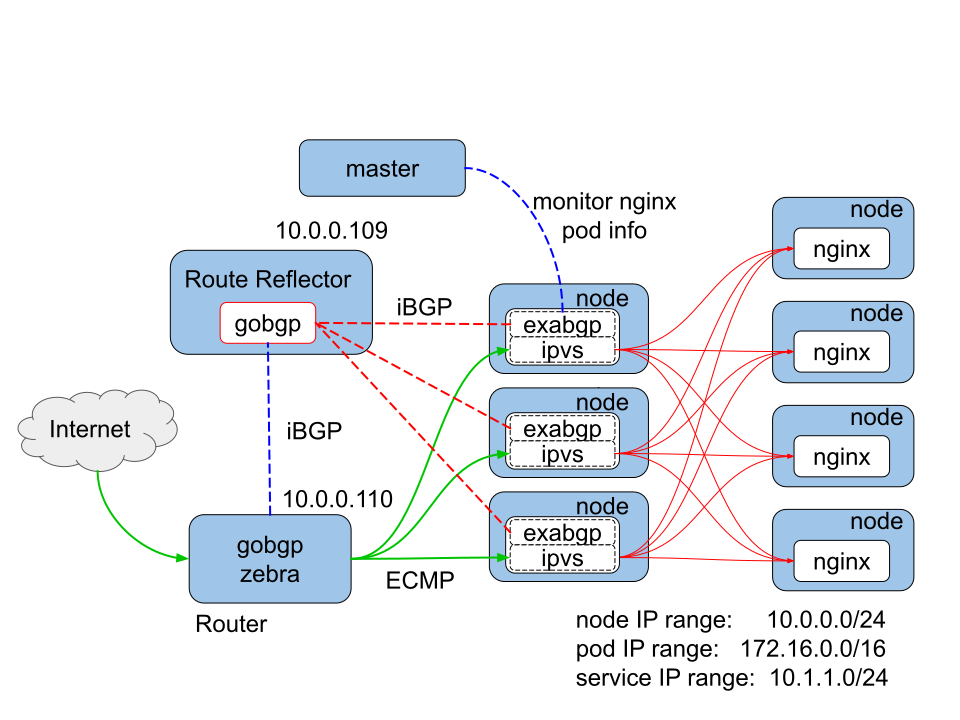
\includegraphics[width=0.8\columnwidth]{Figs/poc.png}
\end{center}
\caption{An experimental container cluster with proposed redundant software balancers}
\centering\parbox[c]{0.9\columnwidth}{
  The master and nodes are configured as Kubernetes's master and nodes on top of conventional Linux boxes, respectively.
  The route reflector and the upstream router are also conventional Linux boxes.
  For the green lines, a service IP address is used. The red lines use the IP addresses of the overlay network. The blue line uses the IP addresses of the node network.
}

\label{fig:poc}
\end{figure}

Fig.~\ref{fig:poc} shows the schematic diagram of proof of concept container cluster system with the proposed software load balancers.
%
Each load balancer pod consists of an exabgp container and an ipvs container.
The ipvs container is responsible for distributing the traffic toward the service IP to web server(nginx) pods.
The IP address for nginx pods and load balancer pods are dynamically assigned upon launch of themselves from 172.16.0.0/16 address range.
The ipvs container monitors the availability of web server pods by consulting apiserver on the master node and manages the load balancing rule appropriately.
The exabgp container is responsible for advertising the route toward the service IP to the route reflector.
The route reflector aggregates the routing information advertised by load balancer pods and advertise them to the upstream router.
The upstream router updates its routing table according to the advertisement.

All the nodes and route reflector are configured using Debian 9.5 with self compiled linux-4.16.12 kernel.  
The author also used conventional Linux box as an upstream router for testing purpose, using the same OS as the nodes and route reflector.
The version of Linux kernel needed to be 4.12 or later to support hash based ECMP routing table.
The author also needed to enable kernel config option CONFIG\_IP\_ROUTE\_MULTIPATH\cite{ipsysctl} when compiling, and set the kernel parameter fib\_multipath\_hash\_policy=1 at run time.
Although in the actual production environment, proprietary hardware router with the highest throughput is usually deployed, one can still test some of the advanced features by using a Linux box as the router.

\begin{table}[H]
  \centering
  \begin{tabular}{|l|c|c|c|}
    \hline
    & \multicolumn{1}{c|}{gobgp} & \multicolumn{1}{c|}{exabgp} & \multicolumn{1}{c|}{bird} \\ \hline
    \begin{tabular}{l} Static route advertisement\\ without injector$^{*}$ \end{tabular} & No  & Yes & No \\ \hline
    \begin{tabular}{l} add-path support$^{**}$ \end{tabular} & Yes & No & Yes  \\ \hline
    \begin{tabular}{l} FIB manupilation \end{tabular} & Yes(through zebra) & No & Yes(Native) \\ \hline
    \begin{tabular}{l} Use case \end{tabular} & Router/Route reflector & Load balancer & Not used$^{***}$  \\ \hline
  \end{tabular}
  \caption{Comparison of open source BGP agents}
  \centering\parbox[c]{0.9\columnwidth}{
    Open source BGP agents are compared in terms of the features required in the proposed systems. \par
    \small
    $^{*}$ \phantom{$^{**}$} The injector is a program that injects static route, other than the BGP daemon itself. \par
    $^{**}$ \phantom{$^{*}$} The add-path is the feature to support multipath advertisement. \par
    $^{***}$ \phantom{$^{}$} Configuration of bird was more omplex than other agents.
  }
  \label{table:bgp_agents}
\end{table}

Table~\ref{table:bgp_agents} compares open source BGP agents in terms of required features for the proposed architecture.
Each load balancer {\em pod} needs to advertise a static route for the service IP to itself. 
For that purpose, exabgp is preferable due to its simplicity.
As for the route reflector, add-path\cite{rfc7911} feature is needed for multi-path advertisement, which is supported by gobgp.
For the upstream router Forwarding Information Base(FIB) manipulation\cite{exa-networks_2018} feature is needed, which is supported by gobgp.
As a result, exabgp is used for the load balancer pods, and gobgp is used for the route reflector and the upstream router.

The other features needed for the route reflector are a dynamic-neighbor feature to describe peer group as a range of IP address, and overlay network feature on the Linux box.
The configurations for the upstream router is summarised in \ref{appendix:router_config}.
The configurations for the route reflector is summarised in \ref{appendix:route_reflector_config}.

\subsection{Ipvs container}\label{sec:ipvs}

The proposed load balancer needs to dynamically reconfigure the ipvs balancing rules whenever {\em pods} are created or deleted. 
Fig.~\ref{fig:ipvs-ingress-schem} is a schematic diagram of ipvs container to show the dynamic reconfiguration of the ipvs rules.
Two daemon programs, controller and keepalived, running in the container are illustrated.
The keepalived manages Linux kernel's ipvs rules depending on the ipvs.conf configuration file.
It can also periodically health check the liveness of a {\em real server}, 
which is represented as a combination of the IP addresses and port numbers of the target {\em pods}. 
If the health check to a {\em real server} fails, keepalived will remove that {\em real server} from the ipvs rules immediately.
The interval of the health check is typically 1 to several seconds and is arbitrarily determined by users.  

\begin{figure}[h]
  \begin{center}
    \includegraphics[width=0.8\columnwidth]{Figs/ipvs-ingress-schem}
    \caption{Implementation of ipvs container.}
    \label{fig:IPVS-ingress-schem}

    \parbox[c]{0.9\columnwidth}{
      The controller checks the pod status every second, by consulting the master node.
      Upon a change of the status, the controller updates the ipvs.conf and sends SIGHUP to keepalived.
      The keepalived reload the ipvs.conf and updates the load balancing rules in the kernel correctly.
    }
  \end{center}

\end{figure}

Every second, the controller monitors information concerning the running {\em pods} of a web application in the Kubernetes cluster by consulting the apiserver running in the master through its API.
Whenever {\em pods} are created or deleted, the controller notices the change and automatically regenerate an appropriate ipvs.conf 
and issue SIGHUP to keepalived within a second.
Then, keepalived will reload the ipvs.conf, and modify the kernel's ipvs rules correctly depending on the result of the health check.

When a pod is terminated, existing connections are reset by the node kernel.
The SYN packets sent to a pod after termination, but before the ipvs rule update, will be answered with ICMP unreachable by the node.
In these cases, the client sees connection errors.
In order to avoid the connection errors to be seen by a human, HTTP client programs are required to re-initiate the connection.
However, since the load balancer rule update is within a second, these errors can be regarded as the tolerable rare exceptions even without such re-initiations.

The actual controller\cite{ktaka_ccmp_2017_826894} is implemented using the Kubernetes ingress controller\cite{K8sIngress2017} framework. 
By importing existing Golang package, \enquote{k8s.io/ingress/core/pkg/ingress}, the author could simplify the implementation, e.g. 
120 lines of code.  
%
Keepalived and the controller are placed in the docker image of ipvs container.
The ipvs is the kernel function and namespace separation for container has already been supported in the recent Linux kernel. 

Configurations for capabilities were needed when deploying the ipvs container: adding the CAP\_SYS\_MODULE capability 
to the container to allow the kernel to load required kernel modules inside a container, 
and adding CAP\_NET\_ADMIN capability to the container to allow keepalived to manipulate the kernel's ipvs rules. 
For the former case, the author also needed to mount the \enquote{/lib/module} of the node's file system on the container's file system.

\begin{figure}[h]
  \centering
  \begin{minipage}{0.7\columnwidth}
    \begin{lstlisting}[frame=single]
      virtual_server fwmark 1 {
        delay_loop 5
        lb_algo lc
        lb_kind NAT
        protocol TCP
        real_server 172.16.21.2 80 {
          uthreshold 20000
          TCP_CHECK {
            connect_timeout 5
        connect_port 80
          }
        }
        real_server 172.16.80.2 80 {
          uthreshold 20000
          TCP_CHECK {
            connect_timeout 5
            connect_port 80
          }
        }
      }
    \end{lstlisting}
  \end{minipage}

  \caption{An example of ipvs.conf}
  \label{fig:ipvs.conf}

  \begin{minipage}{0.9\columnwidth}
    This configuration file is auto-generated by the controller.
    The controller periodically accesses the apiserver on the master node and constantly monitor the status of running pods.
  \end{minipage}
\end{figure}

\begin{figure}[h]
  \centering
  \rule{\columnwidth}{0.4pt}
\begin{verbatim}
# kubectl exec -it IPVS-controller-4117154712-kv633 -- IPVSadm -L
IP Virtual Server version 1.2.1 (size=4096)
Prot LocalAddress:Port Scheduler Flags
  -> RemoteAddress:Port Forward Weight ActiveConn InActConn
FWM  1 lc
  -> 172.16.21.2:80      Masq    1      0          0         
  -> 172.16.80.2:80      Masq    1      0          0
\end{verbatim}
\rule{\columnwidth}{0.4pt}

\caption{Example of IPVS balancing rules}
\label{fig:IPVS rule}

\begin{minipage}{0.9\columnwidth}
  This shows the load balancing rule in a load balancer container.
  The packet that has FWM(fwmark)=1 will be forwarded to two real servers using the least connection(lc) balancing algorithm.
  The fwmark is a parameter that is only available inside a socket buffer in Linux kernel.
  The fwmark can be put and manipulated by the iptables program, once a socket buffer for a received packet is assigned by the kernel.
\end{minipage}
\end{figure}

Figure~\ref{fig:ipvs.conf} and Figure~\ref{fig:IPVS rule} show an example of an ipvs.conf file 
generated by the controller and the corresponding IPVS load balancing rules, respectively.
Here, we can see that the packet with {\tt fwmark=1}\cite{BertHubert2002} is distributed 
to {\tt 172.16.21.2:80} and {\tt 172.16.80.2:80} 
using the masquerade mode(Masq) and 
the least connection(lc)\cite{Zhang2000} balancing algorithm.

\subsection{BGP software container}\label{sec:bgp}

\begin{figure}[tb]
  \begin{center}
    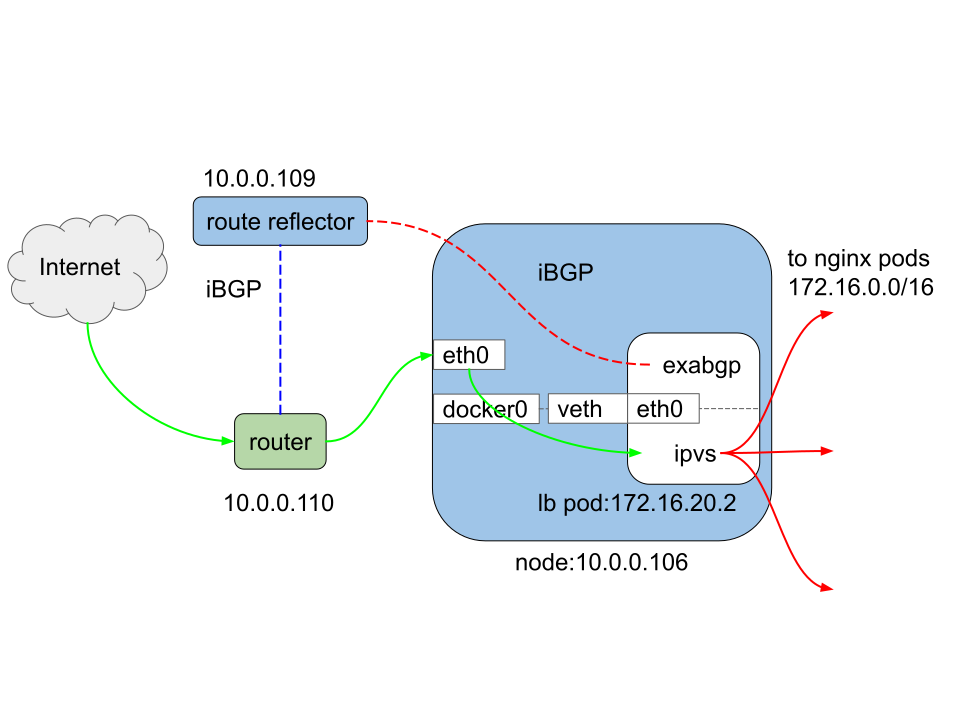
\includegraphics[width=0.8\columnwidth]{Figs/exabgp}
    \caption{Network path by the exabgp container}
    \label{fig:exabgp_schem}
  
    \parbox[c]{0.9\columnwidth}{
      The packets from Internet to service IPs, 10.1.1.0/24 are routed to the load balancer pod(green arrows) by the set of routing rules shown in Table~\ref{table:exabgp_setting}.
      And then the ipvs container forwards them to nginx pods(red arrows).
      The IP address of any pod is dynamically assigned from 172.16.0.0/16 when the pod is started. 
    }
  \end{center}
\end{figure}

\begin{table}
  \begin{center}
    \begin{tabular}{lllr}
      \hline 
      \multicolumn{4}{l}{[BGP announcement]} \\
      \hspace{15 mm} & \multicolumn{2}{l}{route 10.1.1.0/24 next-hop 10.0.0.106} & ...(1) \\
      \multicolumn{4}{l}{[Routing in node net namespace]} \\
      \hspace{15 mm} & \multicolumn{2}{l}{ip netns exec node ip route replace 10.1.1.0/24 dev docker0} & ...(2) \\
      \multicolumn{4}{l}{[Accept as local]} \\
      \hspace{15 mm} & \multicolumn{2}{l}{ip route add local 10.1.1.0/24 dev eth0} & ...(3) \\
      \hline
    \end{tabular}
    \caption{Required settings in the exabgp container}
    \label{table:exabgp_setting}
  
    \parbox[c]{0.9\columnwidth}{
      (1) The node IP address, 10.0.0.106 is used as next-hop for the service IPs, 10.1.1.0/24, in BGP announcement.
      (2) In order to route the packets destined toward the service IP to the container, a routing rule to the dev docker0 is created in the node net namespace. 
      (3) A routing rule to accept the packets destined toward the service IPs,  as local is also required.
    }
  \end{center}
\end{table}

In order to implement the ECMP redundancy, the author also containerized exabgp using Docker.
Figure~\ref{fig:exabgp_schem} shows a schematic diagram of the network path realized by the exabgp container.
As mentioned earlier, the author used exabgp as the BGP advertiser. 
The ingress traffic from the Internet is forwarded by ECMP routing table on the router to the node that hosts a load balancer pod.
And then it is routed to the load balancer pod according to the set of routing rules in Figure~\ref{fig:exabgp_schem}.
After that the ipvs forwards them to nginx pods.
The IP address of any pod is dynamically assigned from 172.16.0.0/16 when the pod is started. 

Table~\ref{table:exabgp_setting} summarises some key settings required in the exabgp container to route the traffic to the ipvs container.
In BGP announcements the node IP address, 10.0.0.106 is used as the next-hop for the service IPs, 10.1.1.0/24.
Then on the node, in order to route the packets toward the service IPs to the ipvs container, 
a routing rule for 10.1.1.0/24 to the dev docker0 is created in the node net namespace. 
A routing rule to accept the packets toward the service IPs as local is also required in the container net namespace. 
A configuration for exabgp is shown in \ref{appendix:exabgp_config}.

\FloatBarrier

\mytodo[inline]{Add a mention about ingress controller implementation, if possible.}


\section{Summary}
In this chapter the author provided discussion of load balancer architecture and its implementations suitable for container clusters.

First the author discussed problems of conventional architecture. 
Since Kubernetes is dependent on external load balancers provided by the cloud infrastructures, 
it failed to provide portability of a web application in environments where there was no supported load balancer. 
Furthermore the routes ingress traffic from the internet follow were very complex and inefficient.

In order to alleviate these problems, the author proposed a cluster of software load balancers in containers.
The proposed load balancers utilized container technotlogy and was managed by Kubernetes.
As a result, it is runnable on any environment including cloud infrastructures and on-premise data centes.
Furthermore, since Kubernetes manages load balancer containers, it can quickly scale the number containers depending on the demand.

The author also discussed redundant architecture using ECMP with BGP for proposed load balancer containers.
By using the ECMP, the upstream router can route the ingress traffic to a cluster of load balancer containers in a redundant and scalable mannar.
By using BGP, which is the standard protocol, ECMP routing rules in the upstream router are automatically populated, upon the launch of load balancer containers.

As a result users, i.e., web application providers can quickly and automatically set up routes to their web application, upon its launch.
This will greatly improve the portability of a web application and there by enables migrations.




\chapter{Performance Evaluation}\label{chapter:Performance Evaluation}

In order to verify the feasibility of the proposed load balancer architecture, the author evaluated the performance of the load balancer with the following criteria;
(1) Performance analysis:
The author evaluated the basic characteristics of the load balancer using physical servers in the on-premise data center, and compared performance level with existing iptables DNAT and nginx as a load balancer.
(2) Portability:
The author also carried out the same performance measurement in GCP and AWS to show the containerized ipvs load balancer is runnable even in the cloud environment.
(3) Redundancy and Scalability:
The author evaluated ECMP functionality by watching routing table updates on the router when the new load balancer is added or removed.
The author also evaluated the performance level by changing the number of load balancers.

\section{Performance analysis of proposed load balancer}

Throughput measurements were carried out in order to examine the basic characteristics of the containerized ipvs load balancer in an on-premise data center.
Figure~\ref{fig:benchmark-schem} shows the schematic diagram of the experimental setup for the measurement.
A benchmark program called wrk\cite{Glozer2016} were used.
Multiple nginx {\em pods} are deployed on multiple nodes as web servers in the Kubernetes cluster.
In each nginx {\em pod}, single nginx web server that returns the IP address of the {\em pod} is running.
The author then launched ipvs, and nginx load balancers on one of the nodes, and performed the throughput measurement changing the number of the nginx pods.
The throughput is measured by sending out HTTP requests from the wrk towards a load balancer and by counting the number of responses the benchmark host received.
On a Kubernetes node there are iptables DNAT rules that functions as the internal load balancers.
The throughput is also measured for the iptables DNAT as a load balancer.

\begin{figure}[h]
  \centering
  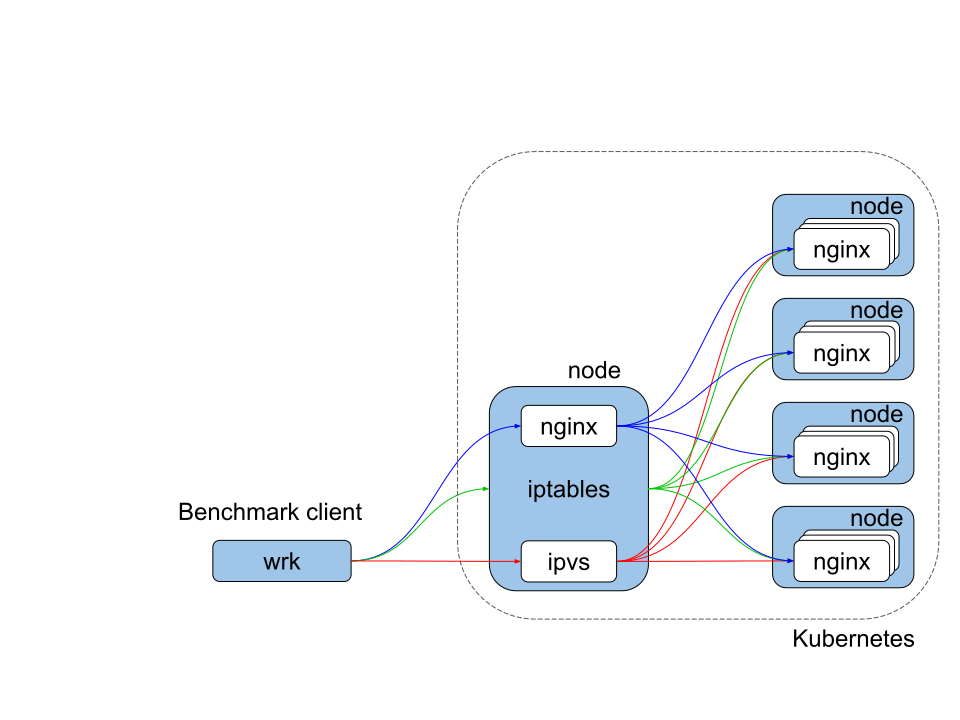
\includegraphics[width=0.9\columnwidth]{Figs/benchmark-schem}
  \caption[Benchmark setup]{Benchmark setup}
  \label{fig:benchmark-schem}
\end{figure}

Figure~\ref{fig:benchmark-schem} shows an example of the command-line for the benchmark program, wrk and the corresponding output.
The command-line in Table~\ref{tab:bench_example} will generate 40 wrk program threads
and allow those threads to send out a total of 800 concurrent HTTP requests over the period of 30 seconds.
The output example shows information including per-thread statistics, error counts, throughput in [Request/sec] and data rate in [Transfer/sec].

\begin{table}[h]
  \centering
  \begin{tabular}{l}
    \hline
    \begin{minipage}{0.7\columnwidth}
      \begin{verbatim}

[Command line] 
 wrk -c800 -t40 -d30s http://172.16.72.2:8888/ 
-c: concurrency, -t: # of thread, -d: duration 

[Output example] 
 Running 30s test @ http://10.254.0.10:81/ 
  40 threads and 800 connections 
  Thread Stats   Avg      Stdev     Max   +/- Stdev 
    Latency    15.82ms   41.45ms   1.90s    91.90\% 
    Req/Sec     4.14k   342.26     6.45k    69.24\% 
  4958000 requests in 30.10s, 1.14GB read 
  Socket errors: connect 0, read 0, write 0, timeout 1 
Requests/sec: 164717.63 
Transfer/sec:     38.86MB 
      \end{verbatim}
    \end{minipage}
    \\ \hline
  \end{tabular}
  \caption[Benchmark command line and output example]{Benchmark command line and output example.}
  \label{tab:bench_example}
\end{table}

{
\setlength{\tabcolsep}{3em}
\renewcommand{\arraystretch}{1.1}

\begin{table}[h]
  \centering
  \begin{tabular}{ll}
    \hline 
    \multicolumn{2}{l}{[Hardware Specification]}   \\
    & CPU: Xeon E5-2450 2.10GHz (with 8 core, Hyper Threading) \\
    & Memory: 32GB \\
    & NIC: Broadcom BCM5720 with 4 rx-queues, 1 Gbps \\
    & (Node x 6, Load Balacner x 1, Client x 1) \\
    & \\
    \multicolumn{2}{l}{[Node Software]}  \\
    & OS: Debian 8.7, linux-3.16.0-4-amd64 \\
    & Kubernetes v1.10.6 \\
    & flannel v0.7.0 \\
    & etcd version: 3.0.15 \\
    & \\
    \multicolumn{2}{l}{[Container Software]}   \\
    & Keepalived: v1.3.2 (12/03,2016) \\
    & nginx : 1.11.1(load balancer), 1.13.0(web server) \\
    \hline
  \end{tabular}
  \caption[Hardware and software specifications]{Hardware and software specifications.}
    \label{tab:hw_machine_spec}
\end{table}
}

Table~\ref{tab:hw_machine_spec} shows hardware and software configuration used in the experiment.
The author used a total of eight servers; six servers for Nodes, one for the load balancer and one for the benchmark client, with all having the same hardware specifications.
The hardware had eight physical CPU cores and a NIC with 4 rx-queues.
The author configured nginx HTTP server to return a small HTTP content, the IP address of the {\em pod}, to make a relatively severe condition for load balancers. 
The size of the character string making up an IP address is limited to 15 bytes.

The author also investigated the performance level, varying two types of network configurations:
The first is the setting for multicore packet processing.
It is known that distributing handling of interrupts from the network interface card (NIC) and the subsequent IP protocol processing, among multiple cores impact the network performance.
In order to derive the best performance from load balancers, the author investigated how this setting would affect their performance.
The other one is an overlay network setting\cite{Sill2016,Marmol2015} that is often used to build the Kubernetes cluster.
Flannel\cite{CoreOSFlannel} is one of the popular overlay network technologies. 
The author compared the performance levels of three backends settings\cite{CoreOSFlannelBackend}, i.e., operating modes of flannel, to find the best setting.

\FloatBarrier

\subsection{Effect of multicore proccessing}

Figure~\ref{fig:ipvs_mcore_proccessing} shows a result of the throughput measurement for ipvs and iptables DNAT.
with different multicore proccessing settings, where 1, 4, 8 cores are utilized respectively.

The following three RSS and RPS settings were compared: 
\begin{center}
  \centering
  \begin{minipage}{0.8\columnwidth}
\begin{verbatim}
(RSS, RPS) = (off, off)
           = (on , off)
           = (off, on )
\end{verbatim}
  \end{minipage}
\end{center}

Since hardware used in the experiment has a NIC with 4 rx-queues, and a cpu with 8 cores,
\enquote{(RSS, RPS) = (off, off)} uses only one core for the packet proccessing,
\enquote{(RSS, RPS) = (on, off)} uses 4 cores and \enquote{(RSS, RPS) = (off, on)} uses 8 cores. 

%% The case with \enquote{(RSS, RPS) = (off, off)} means that multicore packet processing is completely disabled, i.e.,  all the incoming packets are processed by a single core.
%% The \enquote{(RSS, RPS) = (on, off)} means that the interrupt handling and the following IP protocol processing are performed on four of the CPU cores by assigning four rx-queues to those cores. In this case four of the eight CPU cores are utilized.
%% The \enquote{(RSS, RPS) = (off, on)} means that a single core handles all of the interrupts from the NIC then the following IP processings are performed on the other cores. In this case, all of the eight CPU cores are utilized.

\begin{figure}[h]
  \begin{subfigure}[t]{\columnwidth}
    \centering
    \includegraphics[width=0.9\columnwidth]{Figs/ipvs_mcore_proccessing}
    \caption{ipvs}
    \label{fig:ipvs_mcore_proccessing}
  \end{subfigure}

  \par\bigskip

  \begin{subfigure}[t]{\columnwidth}
    \centering
    \includegraphics[width=0.9\columnwidth]{Figs/iptables_mcore_proccessing}
    \caption{iptables DNAT}
    \label{fig:iptables_mcore_proccessing}
  \end{subfigure}

  \centering
  \begin{minipage}{0.9\columnwidth}
    \caption[Effect of multicore proccessing]{
      Effect of multicore proccessing on throughput.
      For both ipvs and iptables DNAT, throughput increases with more cores used.
    }
    \label{fig:effect_of_mcore_proccessing}
  \end{minipage}

\end{figure}

There is a general trend in which the throughput linearly increases as the number of nginx {\em pod}s increases and then it eventually saturates.
The saturated throughput levels indicate the maximum performance level of the ipvs load balancer.

The maximum performance levels depend on the number of cores used for packet proccessing.
It is clear that the case that utilizes all of the CPU cores better performs than the case with only four CPU cores utilized. 

\FloatBarrier

\subsection{Effect of overlay network}

\begin{figure}[h]
  \begin{subfigure}[t]{\columnwidth}
    \centering
    \includegraphics[width=0.9\columnwidth]{Figs/ipvs_flannel_mode}
    \caption{Effect of flannel backend modes on ipvs throughput.}
    \label{fig:ipvs_flannel_mode}
  \end{subfigure}

  \par\bigskip

  \begin{subfigure}[t]{\columnwidth}
    \centering
    \includegraphics[width=0.9\columnwidth]{Figs/iptables_flannel_mode}
    \caption{Effect of flannel backend modes on iptables throughput.}
    \label{fig:iptables_flannel_mode}
  \end{subfigure}

  \centering
  \begin{minipage}{0.9\columnwidth}
    \caption[Effect of flannel backend modes]{
      Effect of flannel backend modes.
      For both ipvs and iptables DNAT,
      the host-gw mode where no encapsulation is conducted shows the highest performance level,
      followed by the vxlan mode where the Linux kernel encapsulate the Ethernet frame.
      The udp mode where flanneld itself encapsulate the IP packet shows significantly lower performances levels, for bose load balancers.
    }
    \label{fig:effect_of_flannel_mode}
  \end{minipage}

\end{figure}

Figure~\ref{fig:ipvs_flannel_mode} shows the ipvs throughput results for different overlay network settings.
The author used the flannel for the overlay network.
Flannel has three backend modes, host-gw, vxlan and udp, and the throughput for each setting are compared.

Except for the udp backend mode case, a general trend can be seen, i.e., the throughput linearly increases as the number of nginx {\em pod} increases, and then it eventually saturates.
The saturated throughput levels indicate the maximum performance levels of the ipvs load balancer.
Among the flannel backend mode types, the host-gw mode where no encapsulation is conducted shows the highest performance level,
followed by the vxlan mode where the Linux kernel encapsulates the Ethernet frame.
The udp mode where flanneld itself encapsulates the IP packet shows significantly lower performances levels.
The author considers the host-gw mode is the best, the vxlan tunnel the second best and the udp tunnel mode unusable.
As is shown here, overlay network settings greatly affect the performance level.
The author used host-gw mode for the rest of the experiments conducted in on-premise data centers and vxlan mode for the experiments conducted in cloud environments.

\FloatBarrier

\subsection{Comparison of different load balancer}

\begin{figure}[h]
  \includegraphics[width=0.9\columnwidth]{Figs/ipvs-iptables-nginx}
  \caption{Throughput measurement results of the proposed load balancer in on-premise data center.}
  \label{fig:ipvs-iptables-nginx}
\end{figure}

\interfootnotelinepenalty=10000

Fig.~\ref{fig:ipvs_performance}~(\subref{fig:ipvs-iptables-nginx}) shows the throughput of the proposed ipvs container load balancer.
The performance of the nginx and the iptables DNAT as the load balancers are also presented for comparison.
As we increased the number of the nginx pods(web servers) from 1 to around 14, the throughput increased almost linearly and after which it saturated.
The increase indicates that the load balancer functions properly because it increased throughput by distributing HTTP requests to multiple of the web servers.
The saturated performance level indicates the maximum performance of the load balancer, which could be determined either by network bandwidth or CPU performance level of the load balancer or the benchmark client.
In this specific experiment, the performance level was limited by the 1 Gbps bandwidth of experimental network\cite{takahashi2018portable}, which is revealed by packet level analysis using tcpdump.
On average the data size of each request and the corresponding response was about 636 [byte/req] in total, including TCP/IP headers, Ethernet header, and inter frame gaps.
Multiplying that with 190K [req/sec] and 8 [bit/byte] will result in 966.72 Mbps.

While nginx did not show any benefit as the load balancer, the performance of the ipvs load balancer container showed equivalent performance level as the un-containerized iptables DNAT.
This means that our proposed ipvs container load balancer is at least as good as the un-containerized iptables' load balancing in the 1 Gbps network.

\subsection{Comparison of different load balancer}

\begin{figure}[h]
  \centering
  \includegraphics[width=0.8\columnwidth]{Figs/ipvs-iptables-nginx}
  \caption{Throughput comparison between ipvs, iptables DNAT and nginx.}
  \label{fig:ipvs-iptables-nginx}
\end{figure}

Figure~\ref{fig:ipvs-iptables-nginx} compares the performance measurement results for different load balancer ipvs, iptables DNAT, and nginx.
The proposed ipvs load balancer exhibits almost equivalent performance levels as the iptables DNAT based load balancer. 
The nginx based load balancer shows no performance improvement even though the number of the nginx web server {\em pods} is increased.
It is understandable because the performance of the single nginx as a load balancer is expected to be similar to the performance as a web server.

\begin{figure}[h]
  \centering
  \includegraphics[width=0.8\columnwidth]{Figs/tp_limit_1gbps}
  \caption{Performance limit due to 1Gbps bandwidth}
  \label{fig:performance_limit}
\end{figure}

At first, it was not clear what caused the performance limit for the case when \enquote{(RSS, RPS) = (off, on)},
the author thought it was due to the insufficient CPU performance.
However, that was not the case in the conditions of the experiment; it turned out to be due to the 1Gbps bandwidth.
A packet level analysis using tcpdump\cite{jacobson1989tcpdump} revealed that 665.36 bytes of extra HTTP headers,
TCP/IP headers and ethernet frame headers are needed for each request in the case of the wrk benchmark program(Appendix~\ref{appendix:performance_limit}).
This results in the upper limit of 184,267 [req/sec] when the date size of HTTP response body is 13 byte, which agrees well with the performance limit for the case when \enquote{(RSS, RPS) = (off, on)} in Figure~\ref{fig:ipvs_mcore_proccessing}.
Figure~\ref{fig:performance_limit} shows the theoretical upper limit of the performance level for 1Gbps ethernet together with actual benchmark results for the range of larger data sizes, and they agree very well.
Therefore it can be said that when \enquote{RPS = on}, ipvs performance is limited by 1Gbps bandwidth.
The author regarded that \enquote{(RSS, RPS) = (off, on)} is the best setting in our experimental conditions, and used this setting throughout this thesis unless explicitly stated otherwise.

\begin{figure}[h]
  \centering
  \includegraphics[width=0.8\columnwidth]{Figs/latency_cdf_rps_40pods}
  \caption{Latency cumulative distribution function.}
  \label{fig:latency_cdf_rps_40pods}
\end{figure}

Figure~\ref{fig:latency_cdf_rps_40pods} compares Cumulative Distribution Function(CDF) of the load balancer latency at the two constant loads, 160K[req/sec] and 180K[req/sec] for ipvs and iptables DNAT.
We can see that the latencies are a little bit smaller for ipvs.
For example, the median values at 160K[req/sec] load for ipvs and iptables DNAT are, 1.14 msec and 1.24 msec, respectively.
Also, at 160K[req/sec], they are 1.39 msec and 1.45 msec, respectively.
These may not be considered a significant difference; however, we can at least say that our proposed load balancer is as good as iptables DNAT.
So, to conclude this section, the containerized ipvs load balancer showed equivalent performance levels with the iptables DNAT load-balancing function that is used in Kubernetes cluster.

%\subsection{Resource Consumption}

Fig.~\ref{fig:cpu_usage} compares the CPU usage for proposed load balancer(ipvs in a container) and iptables DNAT at the time of the throughput measurement in the on-premise data center.
Since the CPU usage was higher for the ipvs in a container, the proposed load balancer may be less efficient compared with the iptables DNAT.
%The proposed architecture requires additional computational resources compared with the conventional architecture.
However since single hardware can accommodate 1 Gbps traffic with CPU usage of about 60\%, the authors regard this as a tolerable overhead.
The authors plan to improve the efficiency of the proposed load balancer by developing a software load balancer using eXpress data path(XDP) technology\cite{hoiland2018express} in the future work and thereby improving the performance levels of the portable load balancer.

\begin{figure}[h]
  \centering
  \includegraphics[width=0.8\columnwidth]{Figs/cpu_usage}
  \caption{CPU usage of the ipvs and iptables DNAT.}
  \label{fig:cpu_usage}
\end{figure}


\FloatBarrier

\subsection{L3DSR using ipvs tun}

The performance levels of ipvs and iptables DNAT have been limited by 1 Gbps bandwidth.
This can be alleviated in the case of ipvs by using so-called Layer 3 Direct Server Return(l3dsr) setup.
Figure~\ref{fig:benchmark-schem-dsr} shows the schematic diagram illustrating packet flow for the HTTP request packet(the red arrows) and response packet(the blue arrow).

\begin{figure}[h]
  \centering
  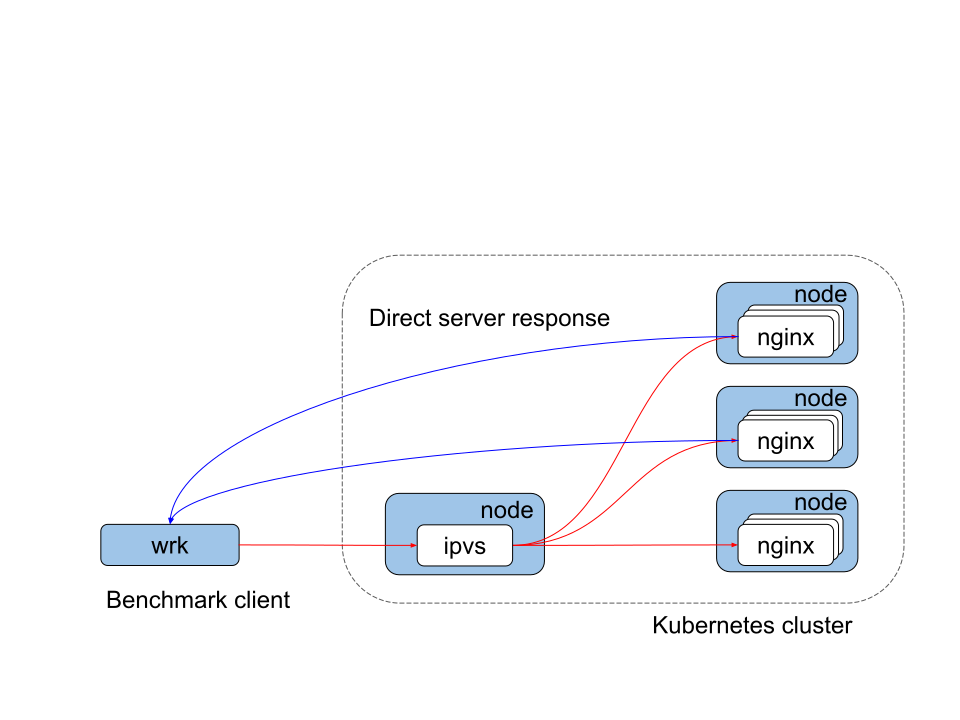
\includegraphics[width=0.8\columnwidth]{Figs/benchmark-schem-dsr}
  \caption{Physical configuration for L3DSR experiment.}
  \label{fig:benchmark-schem-dsr}
\end{figure}

The ipvs has the mode called ipvs-tun.
When the ipvs-tun send out the packets to real servers, it encapsulates the original packet in ipip tunneling packet that is destined to real servers.
The real server receives the packet on a tunl0 device and decapsulates the ipip packet, revealing the original packet.
Since the source IP address of the original packet is maintained, the returning packets are sent directly toward the benchmark client.
In this scheme, the returning packets do not consume the bandwidth nor the CPU power of the load balancer node.

The iptables DNAT does not have the functions that enable L3DSR settings.
Therefore this one of the benefits of the ipvs load balancer.

\begin{figure}[h]
  \centering
  \includegraphics[width=0.8\columnwidth]{Figs/ipvs_l3dsr_1g.png}
  \caption{Throughput of ipvs l3dsr @1Gbps.}
  \label{fig:ipvs_l3dsr_1g.png}
\end{figure}

The author carried out throughput measurement using the physical setup shown in Figure~\ref{fig:bench_1g_l3dsr}.
Figure~\ref{fig:ipvs_l3dsr_1g.png} shows the throughput of the ipvs-tun, conventional ipvs (after here the author call it ipvs-nat) and iptables DNAT.
As can be seen in the figure, while the performance levels for ipvs-nat and iptables DNAT exactly match, the performance levels for ipvs-tun is greatly improved, e.g., 1.5 times larger saturated throughput than for ipvs-nat and iptables DNAT cases.

\FloatBarrier

%\section{IEICE}

\section{Cloud Experiment}

Throughput were also measured in the cloud.

{
\setlength{\tabcolsep}{3em}
\renewcommand{\arraystretch}{1.1}

\begin{table}[h]
  \centering
  \begin{tabular}{ll}
    \hline 
    \multicolumn{2}{l}{[GCP VM Instance Specification]}   \\
    & Instance type: custom instance \\
    & CPU: Xeon 2.2GHz, 8, 16, 32 cpus \hspace{2cm} \\
    & Memory: 16GB \\
    & NIC: virtio\_net /w 16 rx-queues, 1Gbps \\
    & (Node x 6, Load balancer x 1, Client x 1) \\
    & \\
    \multicolumn{2}{l}{[AWS VM Instance Specification]}   \\
    & Instance type: c4.2xlarge, c4.4xlarge, c4.8xlarge  \\
    & CPU: Xeon E5-2666 v3 2.90GHz, 8, 16, 32 cpus \\
    & Memory: 64GB \\
    & NIC: ixgbevf /w 2 rx-queues, 1Gbps \\
    & (Node x 6, Load balancer x 1, Client x 1) \\
    \hline
  \end{tabular}
  \caption[Virtual Machine specifications]{Virtual Machine specifications.}
  \label{fig:cloud_machine_spec}
\end{table}
}

\begin{figure}[h]

  \begin{subfigure}[t]{\columnwidth}
    \includegraphics[width=0.9\columnwidth]{Figs/gcp_all_ieice}
    \caption{Througput in GCP}
    \label{fig:gcp_all_ieice}
  \end{subfigure}

  \par\bigskip

  \begin{subfigure}[t]{\columnwidth}
    \includegraphics[width=0.9\columnwidth]{Figs/aws_c4_ieice}
    \caption{Througput in AWS}
    \label{fig:aws_c4_ieice}
  \end{subfigure}

  \caption[Throughput measurement results in cloud infrastructures]{Throughput measurement results in cloud infrastructures.}
  \label{fig:cloud_ipvs_performance}

\end{figure}

Fig.~\ref{fig:ipvs_performance}~(\subref{fig:gcp_all_ieice}) and Fig.~\ref{fig:ipvs_performance}~(\subref{fig:aws_c4_ieice}) show the load balancer performance levels that are measured in GCP and AWS, respectively. In the case of GCP, custom instance with 32Gbyte memory and with 8, 16, and 32 CPU are used.
And in the case of AWS instance type of c4.2xlarge, c4.4xlarge, and c4.8xlarge are used.
These are aimed to show that our proposed load balancer can be run in cloud environments and also functions properly.

Both results show similar characteristics as the experiment in an on-premise data center in Fig.~\ref{fig:ipvs_performance}~(\subref{fig:ipvs-iptables-nginx}), where throughput increased linearly to a certain saturation level that is determined by either network speed or machine specifications.
Since in the cases of cloud environments we can easily change the machine specifications, especially CPU counts, we measured throughput with several conditions of them.
From the first look of the results, since changing CPU counts changed the load balancer's throughput saturation levels, we thought VM's computation power limited the performance levels.
However, since there are cases in the cloud environment, where changing the VM types or CPU counts also changes the network bandwidth limit, a detailed analysis is further required in the future to clarify which factor limits the throughput in the cases of these cloud environments.
Still, we can say that the proposed ipvs load balancers can be run in GCP and AWS, and function properly.

\FloatBarrier

\section{Redundancy with ECMP}

The ECMP technique is expected to make the load balancers redundant and scalable since all the load balancer containers act as active.
We examined the behavior of the ECMP routing table updates, by changing the number of the load balancers.
After that, in order to explore the scalability, we also measured the throughput from a benchmark client with ECMP routes when multiple of the ipvs container load balancers are deployed.

\begin{figure}[h]
  \centering
  \includegraphics[width=0.9\columnwidth]{Figs/lb_ecmp_schem}

  \centering
  \begin{minipage}{0.9\columnwidth}
    \caption[Benchmark setup]{Benchmark setup.}
    \label{fig:ecmp-benchmark-schem}
  \end{minipage}
\end{figure}

{
\setlength{\tabcolsep}{1em}
\renewcommand{\arraystretch}{1.2}

\begin{table}[h]
  \centering
  \begin{tabular}{ll}
    \hline 
    \multicolumn{2}{l}{[Hardware Specification]}   \\
    & CPU: Xeon E5-2450 2.10GHz x 8 (with Hyper Threading) \\
    & Memory: 32GB \\
    & NIC: Broadcom BCM5720 Giga bit \\
    & (Node x 6, Load Balancer x 4) \\
    & \\
    & CPU: Xeon E5-2450 2.10GHz x 8 (with Hyper Threading) \\
    & Memory: 32GB \\
    & NIC: Intel X550 \\
    & (Client x 1) \\
    & \\
    \multicolumn{2}{l}{[Node Software]}  \\
    & OS: Debian 9.5, linux-4.16.8 \\
    & Kubernetes v1.5.2 \\
    & flannel v0.7.0 \\
    & etcd version: 3.0.15 \\
    & \\
    \multicolumn{2}{l}{[Container Software]}   \\
    & Keepalived: v1.3.2 (12/03,2016) \\
    & nginx : 1.15.4(web server) \\
  \hline 
  \end{tabular}
  \caption{Hardware and software specifications.}
  \label{tab:ecmp-hw_sw_spec}
\end{table}
}

Fig.~\ref{fig:ecmp-benchmark-schem} shows the schematic diagram of the experimental setup and also summarizes hardware and software specifications.
Notable differences from the previous throughput experiment in Fig.~\ref{fig:benchmark-schem} are as follows;
1) Each load balancer pods now consists of both an ipvs container and an exabgp container.
2) The routing table of the benchmark client is updated by BGP protocol through a route reflector.
3) The NIC of the benchmark client has been changed to 10 Gbps card since now we have multiple of ipvs container load balancers that are capable of filling up 1 Gbps bandwidth.
4) Some of the software have been updated to the most recent versions at the time of the experiment.

\FloatBarrier

{
\setlength{\tabcolsep}{1em}
\renewcommand{\arraystretch}{1.2}

\begin{table}[h]

  \begin{subtable}{.9\textwidth}
    \centering
    \begin{tabular}{l}
    \hline 
    10.1.1.0/24 via 10.0.0.106 dev eth0 proto zebra metric 20 \\
    \hline
    \end{tabular}
    \caption{With single load balancer {\em pod}.}
    \label{tab:single}
  \end{subtable}

  \par\bigskip

\begin{subtable}{.9\textwidth}
  \centering
  \begin{tabular}{ll}
    \hline
    \multicolumn{2}{l}{10.1.1.0/24 proto zebra metric 20 } \\
    \hspace{15 mm}
    & nexthop via 10.0.0.105  dev eth0 weight 1 \\
    & nexthop via 10.0.0.106  dev eth0 weight 1 \\
    & nexthop via 10.0.0.107  dev eth0 weight 1 \\
    \hline
  \end{tabular}
  \caption{With three load balancer {\em pod}s.}
  \label{tab:three}
\end{subtable}

  \par\bigskip

\begin{subtable}{.9\textwidth}
  \centering
  \begin{tabular}{ll}
    \hline
    \multicolumn{2}{l}{10.1.1.0/24 pro to zebra metric 20 } \\
    \hspace{15 mm}
    & nexthop via 10.0.0.107  dev eth0 weight 1 \\
    & nexthop via 10.0.0.105  dev eth0 weight 1 \\
    & nexthop via 10.0.0.106  dev eth0 weight 1 \\
    \multicolumn{2}{l}{10.1.2.0/24 proto zebra metric 20 } \\
    \hspace{15 mm}
    & nexthop via 10.0.0.107  dev eth0 weight 1 \\
    & nexthop via 10.0.0.106  dev eth0 weight 1 \\
    \hline
  \end{tabular}
  \caption{For a service with three load balancer {\em pod}s and a service with two load balancer {\em pod}s.}
  \label{tab:double_svc}
\end{subtable}

\caption{ECMP routing tables.}
\label{tab:exabgp_routing_table}
\end{table}
}

First, we examined ECMP functionality by watching the routing table on the benchmark client.
Fig.~\ref{fig:exabgp_routing_table}~(\subref{fig:single}) shows the routing table entry on the router when a single load balancer pod exists.
From this entry, we can tell that packets toward 10.1.1.0/24 are forwarded to 10.0.0.106 where the load balancer pod is running.
It also shows that this routing rule is updated by zebra.

When the number of the load balancer pods is increased to three, we can see the routing table entry in Fig.~\ref{fig:exabgp_routing_table}~(\subref{fig:three}).
We have three next hops towards 10.1.1.0/24 each of which being the node where the load balancer pods are running.
The weights of the three next-hops are all 1.
The update of the routing entry was almost instant as we increased the number of the load balancers.

Fig.~\ref{fig:exabgp_routing_table}~(\subref{fig:double_svc}) shows the case where we additionally started new service with two load balancer pods with service addresses in 10.1.2.0/24 range.
We could accommodate two different services with different service IPs, one with three load balancers and the other with two load balancers on a group of nodes(10.0.0,105,10.0.0,106,10.0.0,107).
The update of the routing entry was almost instant as we started the load balancers for the second service.

As far as the route withdrawal is concerned, if an exabgp is killed by SIGKILL or SIGTERM the kernel of the node close the BGP connection by sending out a packet with FIN flag to the peer gobgpd on the route reflector, and thus the route is withdrawn immediately.
The gobgp on the route reflector also periodically check the BGP connection, and if the peer exabgp container is unresponsive for more than the specified duration, “hold-time“ setting in gobgpd, it will also terminate the connection and withdraw the route.
The packets arriving within the duration will be dropped.
However, we can set up the “hold-time” short enough so that the retransmitted TCP packets from the client will be forwarded correctly to functioning load balancers.

\FloatBarrier

\begin{figure}[h]
  \centering
  \includegraphics[width=0.9\columnwidth,left]{Figs/ecmp_lb_cubic_ieice}
  \centering
  \begin{minipage}{0.9\columnwidth}
        \caption[Throughput of ECMP redundant load balancer]{
          Throughput of ECMP redundant load balancer.
          The throughputs are measured for a single load balancer(lb x1), two(lb x2), three(lb x3) and four(lb x4) load balancers.
        }
  \end{minipage}
  \label{fig:ecmp_lb_cubic_ieice}
\end{figure}

\begin{figure}[h]
  \centering
  \includegraphics[width=0.98\columnwidth,left]{Figs/ecmp_response_ieice}
  \centering
  \begin{minipage}{0.9\columnwidth}
    \caption[Throughput responsiveness]{
      Throughput responsiveness.
      This shows the throughput responsiveness when the number of the load balancers was changed randomly in every 60 seconds.
    }
  \end{minipage}
  \label{fig:ecmp_response_ieice}
\end{figure}


\begin{figure}[h]
  \includegraphics[width=0.9\columnwidth,left]{Figs/ecmp_delay_histgram_ieice}
  \centering
  \begin{minipage}{0.9\columnwidth}
    \caption[A histogram of the ECMP update delay]{
      A histogram of the ECMP update delay.
      This shows the delays until the number of running ipvs pods is reflected into the routing table on the benchmark client,
    when the number of the ipvs pods is changed randomly every 60 seconds for 20 hours.
    }
  \end{minipage}
  \label{fig:ecmp_delay_histgram_ieice}
\end{figure}

We also carried out throughput measurement to show that our proposed architecture increases the throughput as we increase the number of the load balancers.
Fig.~\ref{fig:ecmp_scalability}~(\subref{fig:ecmp_lb_cubic_ieice}) shows the results of the measurements.
There are four solid lines in the figure, each corresponding the throughput result when there are one through four of the proposed load balancers.
The saturated levels, i.e. performance levels depend on the number of the ipvs load balancer pods(lb x 1 being the case with one ipvs pods, and lb x2 being two of them and as such). The performance level increases linearly as we increases the number of the load balancers up to four of the ipvs load balancers, but did not scale further.
This was because we used up CPU power of the benchmark client since the CPU usage was 100\% when there were more than four load balancers.
We expect that replacing the benchmark client with more powerful machines, or changing the experimental setup so that multiple benchmark clients can access the load balancers through an ECMP router, will improve the performance level further.

Fig.~\ref{fig:ecmp_scalability}~(\subref{fig:ecmp_response_ieice}) shows the throughput measurement results when we periodically changed the number of the load balancers. 
The red line in the figure shows the number of the ipvs load balancer pods, which we changed randomly every 60 seconds.
The blue line corresponds to the resulting throughput.
As we can see from the figure, the blue line nicely follows the shape of the red line.
This indicates that new load balancers are immediately utilized after they are created, and after removing some load balancers, the traffic to them is immediately directed to the existing load balancers.

Fig.~\ref{fig:ecmp_scalability}~(\subref{fig:ecmp_delay_histgram_ieice}) shows histogram of the ECMP update delay, where we measured the delays until the number of running ipvs pods is reflected in the routing table on the benchmark client, as we change the number of the ipvs pods randomly every 60 seconds for 20 hours.
As we can see from the figure, most of the delays are within 6 seconds, and the largest delay during the 20 hours experiment was 10 seconds.
We can conclude that ECMP routing update in our proposed architecture is quick enough.

\FloatBarrier

\section{Summary}\label{Conclusions}

In this paper, we proposed a portable load balancer with ECMP redundancy for the Kubernetes cluster systems that is aimed at facilitating migration of container clusters for web services.
We implemented an experimental web cluster system with multiple of load balancers and web servers using Kubernetes and OSSs on top of standard Linux boxes to prove the functionality of the proposed architecture.
We conducted performance measurements and found that the ipvs based load balancer in container functioned properly both in on-premise data center and cloud environments while it showed the comparable performance levels as the existing iptables DNAT based load balancer.
We also carried out experiments to verify the feasibility of ECMP redundancy in on-premise data center, and revealed that it functions properly with linear scalability up to four load balancers.

The current limitations of this study are;
1) Currently, BGP peering is not supported in GCP and AWS, and thus redundancy is achieved only by route update through cloud API upon the start of a load balancer.
The authors expect the cloud providers to support it in the future.
2) Most of the experiments are in 1Gbps network environments.
For future work, we plan to carry out throughput measurement in 10Gbps network environments and also improve the performance of a single software load balancer on standard Linux box using XDP technology.


\chapter{Further Improvement}\label{chapter:performance}
Up until this chapter most of the experiments are done in 1Gbps network environments.
The proposed load balancers have shown decent performance levels in 1Gbps environment.
However, it is essential to investigate the feasibility of the proposed load balancers in 10Gbps network environments.
In this chapter, the author carries out throughput measurements of ipvs-nat, ipvs-tun, and iptables DNAT in 10Gbps environment.
Then the author improves the performance levels of ipvs-nat and ipvs-tun by setting up these load balancers in the node net namespace.
Also presented is the novel software load balancer using eXpress Data Plane(XDP) technology, as an alternative to ipvs software load balancers.

\section{Throuput of ipvs-nat, ipvs-tun and iptables DNAT}

Figure~\ref{fig:bench_10g} shows the packet flow for ipvs-nat and iptables DNAT, and Figure~\ref{fig:bench_10g_l3dsr} shows that for ipvs-tun.
The 10Gbps NICs are used for benchmark client and the node for the load balancer.
In the case of the ipvs-nat and iptables DNAT, the response packets from nginx pods are returned to the load balancer, and then load balancer returns it to the client.
In contrast, in the case of ipvs-tun, the response packets from nginx pods are directly returned to the client.
Since the load balancer does not have to process the response packet, a better performance level is expected for ipvs-tun.

\begin{figure}[h]
  \centering
  \includegraphics[width=0.8\columnwidth]{Figs/bench_10g}
  \caption{Packet flow of ipvs-nat and iptables DNAT.}
  \label{fig:bench_10g}
\end{figure}

\begin{figure}[h]
  \centering
  \includegraphics[width=0.8\columnwidth]{Figs/bench_10g_l3dsr}
  \caption{Packet flow of ipvs-tun.}
  \label{fig:bench_10g_l3dsr}
\end{figure}

\begin{figure}[h]
  \centering
  \includegraphics[width=0.8\columnwidth]{Figs/ipvs_l3dsr_10g}
  \caption{Throughput of load balancers in 10 Gbps.}
  \label{fig:ipvs_l3dsr_10g}
\end{figure}

Figure~\ref{fig:ipvs_l3dsr_10g} shows the throughput of ipvs-tun, ipvs-nat and iptables DNAT in 10Gbps environment.
We can see the general characteristics of a load balancer where the throughput increases linearly to a certain level as the number of nginx container increases, and then eventually saturates.
These saturation levels are the performance limits of each of the load balancers, which is determined by packet forwarding efficiency or the bandwidth of the network.
The performance limit of the iptables DNAT is close to 780k [req/sec], where the CPU usage of the benchmark client becomes 100\%.

Table~\ref{table:nat_tun_dnat_1g_10g} summarizes the throughput of ipvs-tun, ipvs-nat and iptables DNAT at 40 nginx pods in 10 Gbps and 1 Gbps networks.
By using 10 Gbps network, the performance levels for all of these load balancer are improved.
However, the magnitudes of the improvements are different among the types of the load balancers.
While the throughput of the ipvs-nat is 334833 [req/sec], that of the iptables DNAT is 777640 [req/sec].
This suggests that the packet forwarding of the iptables DNAT is more efficient than that of ipvs-nat.
Although the throughput of the ipvs-tun, 730975 [req/sec] is better than ipvs-nat because of the L3DSR settings, it still falls short of that of iptables DNAT.
It seems that containerized ipvs load balancers are inherently less efficient than the iptables DNAT, which could be attributed to either overhead of container network(veth+bridge) or kernel code for ipvs itself.
In order to investigate this issue, the author conducted a throughput measurement for ipvs-nat and ipvs-tun that are set up in node net namespaces in the next section.

\begin{table}[H]
  \centering
  \begin{tabular}{|l|r|r|}
    \hline
    & \multicolumn{2}{c|}{Throughput {[}req/sec{]}} \\ \hline
    Type of load balancer & \multicolumn{1}{c|}{1Gbps} & \multicolumn{1}{c|}{\cellcolor[HTML]{ECF4FF}10Gbps} \\ \hline
    \multicolumn{1}{c|}{iptables DNAT} & 193198 & \cellcolor[HTML]{ECF4FF}777640 \\ \hline
    \multicolumn{1}{c|}{ipvs-nat} & 195666 & \cellcolor[HTML]{ECF4FF}334833 \\ \hline
    \multicolumn{1}{c|}{ipvs-tun} & 292660 & \cellcolor[HTML]{ECF4FF}730975 \\ \hline
  \end{tabular}
  \caption{Performance levels in 1Gbps and in 10Gbps.}
  \raggedright
  Throughput results of the load balancers at 40 nginx pods from the data for the Figures~\ref{fig:ipvs_l3dsr_1g.png} and \ref{fig:ipvs_l3dsr_10g} are shown.
  \label{table:nat_tun_dnat_1g_10g}
\end{table}

\FloatBarrier
\section{Throuput of ipvs-nat, ipvs-tun and iptables DNAT}

In order to improve the throughput of the ipvs load balancers by removing the overhead of container network, the ipvs load balancers were set up in node net namespaces.
Appendix XXX shows inside of ipvs container script that launches the keepalived in node net namespaces.
By doing so, the load balancing tables are created in the node net namespace.

Figure~\ref{fig:ipvs_node_l3dsr_10g} shows the throughput of ipvs-nat and ipvs-tun in the node namespace together with the throughput of the iptables DNAT.
The throughput of the ipvs-tun is almost identical to that of iptables DNAT, which is limited by CPU power of the benchmark client. 
%
Although the throughput of the ipvs-nat is smaller than that of the iptables DNAT, it is clearly improved from the result in Figure~\ref{fig:ipvs_l3dsr_10g}.

Table~\ref{table:nat_tun_dnat_pod_node} compares the throughput of ipvs load balancers in the pod namespace and in the node namespace at 40 nginx pods.
The thoughput data are taken from the results in the Figures~\ref{fig:ipvs_l3dsr_10g} and \ref{fig:ipvs_node_l3dsr_10g}.
We can see that maximum throughputs can be improved in the case of load balancers in node namespace both for the ipvs-nat and the ipvs-tun.  

\begin{figure}[h]
  \centering
  \includegraphics[width=0.8\columnwidth]{Figs/ipvs_node_l3dsr_10g}
  \caption{Throughput of load balancers in node name space.}
  \label{fig:ipvs_node_l3dsr_10g}
\end{figure}

\begin{table}[h]
  \centering
  \begin{tabular}{|l|r|r|}
    \hline
    & \multicolumn{2}{c|}{Throughput {[}req/sec{]}} \\ \hline
    Type of load balancer & \multicolumn{1}{c|}{pod name space} & \multicolumn{1}{c|}{node name space} \\ \hline
    \multicolumn{1}{c|}{iptables DNAT} & NA & \cellcolor[HTML]{ECF4FF}777640 \\ \hline
    \multicolumn{1}{c|}{ipvs-nat} & \cellcolor[HTML]{ECF4FF}334833 & \cellcolor[HTML]{FFF3F3}699635 \\ \hline
    \multicolumn{1}{c|}{ipvs-tun} & \cellcolor[HTML]{ECF4FF}730975 & \cellcolor[HTML]{FFF3F3}779932 \\ \hline
  \end{tabular}
  \caption{Performance levels in pod namespace and in node namespace.}
  \raggedright
  Throughput results of the load balancers at 40 nginx pods from the data for the Figures~\ref{fig:ipvs_l3dsr_10g} and \ref{fig:ipvs_node_l3dsr_10g} are shown.
  \label{table:nat_tun_dnat_pod_node}
\end{table}

\FloatBarrier
\section{XDP load balancer}

\section{Summary}

In this chapter, the author carried out throughput measurements of ipvs-nat, ipvs-tun, and iptables DNAT in 10Gbps environment.
From the results the general characteristics of a load balancer are observesd.
The throughput increases linearly to a certain level as the number of nginx container increases, and then eventually saturates.
The performance levels for of the load balancers are improved by using 10Gbps network.
However, the throughputs of ipvs-nat and ipvs-tun are smaller than that of iptables DNAT.

Then the author improved the performance levels by setting up ipvs-nat and ipvs-tun load balancers in the node net namespace to remove overhead of the container network.
The throughput of the ipvs-tun became almost identical to that of iptables DNAT, and the throughput of the ipvs-nat also improved to the level close to that of the iptables DNAT.

The authot also presented the novel software load balancer using eXpress Data Plane(XDP) technology, as an alternative to ipvs software load balancers.
And brah brah brah.....





\chapter{Related Work}\label{chapter:related}

This Chapter provides related works and the background information of this study.

\section{Related Work}\label{Related Work}

This section highlights related work, especially that dealing with container cluster migration, 
software load balancer containerization, load balancer tools within the context of the container technology and scalable load balancer in the cloud providers.

\paragraph{\bf Container cluster migration:}

Kubernetes developers are trying to add federation\cite{K8sFederation2017} capability for handling situations 
where multiple Kubernetes clusters\footnote{The {\em Kubernetes cluster} refers to a server cluster 
controlled by the Kubernetes container management system, in this paper.} 
are deployed on multiple cloud providers or on-premise data centers, 
and are managed via the Kubernetes federation API server (federation-apiserver). 
However, how each Kubernetes cluster is run on different types of cloud providers
and/or on-premise data centers, especially when the load balancers of such environments are not supported by Kubernetes, 
seems beyond the scope of that project. 
The main scope of this paper is to make Kubernetes usable in environments 
without supported load balancers by providing a containerized software load balancer.

\paragraph{\bf Software load balancer containerization:}
As far as load balancer containerization is concerned, the following related work has been identified:
Nginx-ingress\cite{Pleshakov2016,NginxInc2016} utilizes the ingress\cite{K8sIngress2017} capability of Kubernetes, 
to implement a containerized Nginx proxy as a load balancer. Nginx itself is famous as a high-performance web server program
that also has the functionality of a Layer-7 load balancer. Nginx is capable of handling Transport Layer Security(TLS) encryption, 
as well as Uniform Resource Identifier(URI) based switching. However, the flip side of Nginx is that it is much slower than Layer-4 switching.
We compared the performance between Nginx as a load balancer and our proposed load balancer in this paper.
%
Meanwhile, the kube-keepalived-vip\cite{Prashanth2016} project is trying to use Linux kernel's ipvs\cite{Zhang2000} 
load balancer capabilities by containerizing the keepalived\cite{ACassen2016}.
The kernel ipvs function is set up in the host OS's net namespaces and is shared among multiple web services,
as if it is part of the Kubernetes cluster infrastructure.
Our approach differs in that the ipvs rules are set up in container's net namespaces 
and function as a part of the web service container cluster itself.
The load balancers are configurable one by one, and are  movable with the cluster once the migration is needed.
The kube-keepalived-vip's approach lacks flexibility and portability whereas ours provide them.
%
The swarm mode of the Docker\cite{DockerCoreEngineering2016,DockerInc2017} also uses ipvs for internal load balancing,
but it is also considered as part of Docker swarm infrastructure, 
and thus lacks the portability that our proposal aims to provide.

\paragraph{\bf Load balancer tools in the container context:}
There are several other projects where efforts have been made to utilize ipvs in the context of container environment.
For example, GORB\cite{Sibiryov2015} and clusterf\cite{Aaltodoc:http://urn.fi/URN:NBN:fi:aalto-201611025433} are daemons 
that setup ipvs rules in the kernel inside the Docker container. 
They utilize running container information stored in key-value storages
like Core OS etcd\cite{CoreOSEtcd} and HashiCorp's Consul\cite{HashiCorpConsul}. 
Although these were usable to implement a containerized load balancer in our proposal, we did not use them, 
since Kubernetes ingress framework already provided the methods to retrieve running container information through standard API.

\paragraph{\bf Cloud load balancers:}

As far as the cloud load balancers are concerned, two articles have been identified.
Google's Maglev\cite{eisenbud2016maglev} is a software load balancer used in Google Cloud Platform(GCP).
Maglev uses modern technologies including per flow ECMP and kernel bypass for user space packet processing.
Maglev serves as the GCP's load balancer that is used by the Kubernetes.
Maglev is not a product that users can use outside of GCP nor is an open source software, while the users need open source software load balancer that is runnable even in on-premise data centers.
Microsoft's Ananta\cite{patel2013ananta} is another software load balancer implementation using ECMP and windows network stack.
Ananta can be solely used in Microsoft's Azure cloud infrastructure\cite{patel2013ananta}.
The proposed load balancer by the author is different in that it is aimed to be used in every cloud provider and on-premise data centers.



\chapter{Conclusion and future work }\label{chapter:conclusion}
\section{Conclusions}\label{Conclusions}

As the web services become an indispensable part of the daily life, portability of the application becomes very important.
%
\added[id=2nd]{In order to improve the portability of web applications consisting of container clusters, container orchestrators need to be able to serve as a uniform platform by functioning as a common middleware.}
\deleted[id=2nd]{Container orchestrators are expected to provide a uniform platform for container clusters and facilitate the migration of web applications consisting of container clusters.}
However, \added[id=2nd]{they fail to do so, because }none of the existing container orchestrators \added[id=2nd]{can fully automate the}\deleted[id=2nd]{ fully supports an automatic} setup of \added[id=2nd]{routes for} ingress traffic\deleted[id=2nd]{ routing} from the Internet\deleted[id=2nd]{, failing to serve as a uniform platform}.


\added[id=2nd]{
To solve this problem, the author proposed an architecture using a portable software load balancer that can run on any infrastructure.
The author proposed a cluster of software load balancers in containers that can be launched as a part of web applications for Kubernetes.
}
%
\added[id=2nd]{The proposed architecture is also capable of setting up the routes for the ingress traffic automatically in a redundant and scalable manner.
  For that purpose, Equal Cost Multi Path(ECMP) routes are populated through Border Gateway Protocol(BGP).
  Since both ECMP and BGP are the standard protocols, they are very likely to be supported by most of the upstream routers.
  By using the proposed architecture, container clusters no longer depend on the load balancers provided by infrastructures.
  And hence, container orchestrators become being able to better serve as a common middleware, which will improve the portability of the web applications consisting of container clusters.
}

\deleted[id=2nd]{In this dissertation, the author addresses this problem by proposing a portable software load balancer that is runnable on any infrastructure and capable of an automatic setup of the ingress traffic routing.
The proposed load balancer architecture utilizes software load balancers with container technology to make the load balancers runnable in any base infrastructure.
It also utilizes ECMP technology to make multiple load balancers active, and thereby to provide redundancy and scalability.
The proposed load balancer standardize the way to route traffic into container clusters, by removing dependencies on load balancers provided by infrastructures.
}

To prove the feasibility of the proposed load balancer architecture, the author has implemented a containerized software load balancer using Linux kernel's \replaced[id=2nd]{IPVS}{ipvs} for Kubernetes\deleted[id=2nd]{ and carried out performance measurements in the 1 Gbps network environment.}\added[id=2nd]{, and carried out experiments with the following criteria:}
\added[id=2nd]{
  1) verify if the proposed load balancer works correctly both in the cloud and the on-premise datacenter.
  2) verify if the proposed load balancer has a sufficient performance level for 1 Gbps and 10 Gbps networks.
  3) verify if the proposed redundancy architecture using ECMP with BGP properly functions.
}

\added[id=2nd]{
From the results of the experiments, it has been shown that the 
}
\deleted[id=2nd]{ The }throughput of the proposed load balancer linearly increases as the number of nginx {\em pod}s increases, and then it eventually saturates, indicating \added[id=2nd]{that} the load balancer functions properly.
It has been \added[id=2nd]{also} shown that the proposed load balancers \replaced[id=2nd]{can run}{are runnable} in an on-premise data center, Google Cloud Platform (GCP) and Amazon Web Service (AWS).
Therefore the proposed load balancers can be said to be portable.

The throughputs of a load balancer are dependent on the settings for multi-core packet processing and the setting for the overlay network.
\added[id=2nd]{To derive the best performance, the author used as many CPU cores as possible for packet processing, and the settings without any packet encapsulation for backend mode of the overlay network.}
\deleted[id=2nd]{It has been shown that the setting with as many CPU cores as possible for packet processing results in better performance.
It has been also shown that the backend mode for the overlay network without any packet encapsulation should be used for the best performance.}
%
\added[id=2nd]{From the experiment in the 1 Gbps network environment, the author obtained the highest throughput for the IPVS-TUN (L3DSR) in a container, which is limited by the bandwidth of the benchmark client.
  Since the benchmark client is placed at the same location where the upstream router exists, the load balancer can be said to have sufficient performance to fill up 1 Gbps network bandwidth.
}
\deleted[id=2nd]{The throughput of the ipvs in a container is equivalent to that of the iptables DNAT as a load balancer, in 1Gbps network environment.
The throughput of the ipvs in a container with Layer 3 Direct Server Return (L3DSR) setting has been about 1.5 times higher than that of existing iptables DNAT rules, which is prepared by Kubernetes's daemons as an internal load balancer.}

\added[id=2nd]{
The author also extended the throughput measurement into the 10 Gbps network environment, in order to verify that proposed software load balancer is capable of providing needed throughput for 10 Gbps environment.
The throughputs of IPVS and IPVS-TUN are smaller than that of iptables DNAT in 10Gbps network, both due to the overhead of the container network and inefficiency in the program itself.
Considering the fact that the throughput of the whole system never exceeds that of the upstream router at the entrance, the load balancers only need to be able to handle at most 2.9M [req/sec] in 10Gbps network.
This can be easily achieved using four of the IPVS-TUN (L3DSR) load balancer container since a single IPVS-TUN in a container can handle 731K [req/sec].
Therefore the author also concludes that although there is a room for improvements the proposed load balancer has sufficient performance for 10 Gbps network environment.
}

The author has also implemented an automatic setup of the ECMP route for ingress traffic.
There, multiple load balancer containers are deployed, and each of them advertises itself as an active next hop of the IP for web application through Border Gateway Protocol (BGP).
The ECMP route makes the load balancers redundant and scalable since all the load balancer containers act as active.
%
The BGP helps automatic setup of the ECMP route.  
The BGP and ECMP are both standard protocols supported by most of the commercial router products.
%
The author verified through experiment that an ECMP route has been automatically created upon launch of a new load balancer container on the upstream router.
The update of the ECMP routing table was correct and quick enough, i.e., within 10 seconds, throughout 20 hours experiment.
The maximum performance levels of the cluster of load balancers have scaled linearly up to four times as the number of the load balancer containers has been increased to four of them.
The maximum aggregated throughput obtained through the experiment is 780k [req/sec], which is limited by the CPU performance of the benchmark client, and therefore can be improved using better hardware in the future experiment.
Therefore the author has proved that proposed load balancer has the capability of the automatic setup of ingress traffic in a redundant and scalable manner.
%
\deleted[id=2nd]{
From these results, the author concludes that the proposed load balancer is portable, redundant and scalable while providing 1.5 times better throughput than iptables DNAT in 1Gbps network environment.
}

\deleted[id=2nd]{
The author also extended the throughput measurement into the 10 Gbps network environment, in order to verify that proposed software load balancer is capable of providing needed throughput for 10 Gbps environment.
The throughputs of ipvs and ipvs-tun are smaller than that of iptables DNAT in 10Gbps network, both due to the overhead of the container network and inefficiency in the program itself.
Considering the fact that the throughput of the whole system never exceeds that of the upstream router at the entrance, the load balancers only need to be able to handle at most 2.9M [req/sec] in 10Gbps network.
This can be easily achieved using four of the ipvs-tun (L3DSR) load balancer container since a single ipvs-tun in a container can handle 731K [req/sec].
Therefore the author also concludes the proposed load balancer has enough performance for 10 Gbps network environment.
}

\added[id=2nd]{Sooner or later, the day when the network in a data center becomes all 100 Gbps will come.}
\deleted{Sooner or later, the day will come when the network in a data center will become all 100 Gbps.
    }
\added{Therefore, in the future,}\deleted{For a faster network,} it \replaced{becomes crucial}{is important} to improve the throughput of portable load balancers by using better container network and implementing more efficient software load balancer itself.
The author leaves these for future work, however, a preliminary result of \added{the latter}\deleted{one of these} has also been presented.
The author has implemented a software load balancer using XDP technology and carried out throughput measurement.
The current implementation does not support multicore packet processing, and hence throughput is limited by the capability of single core processing performance.
\replaced[id=2nd]{Nevertheless}{However}, the obtained throughput about 390K [req/sec] for the XDP load balancer \added[id=2nd]{indicates that this technology} is very promising.
The author estimates that about five of the software load balancer using this technology with 16 core packet processing can provide enough throughput, 29M [req/sec] in 100 Gbps environments in the future. 

The proposed load balancer has been verified to be portable while providing \replaced[id=2nd]{sufficient}{enough} throughput in 10 Gbps environment.
\added[id=2nd]{
  And the proposed redundancy architecture using ECMP with BGP has also been verified to function properly.
  As a consequence, the proposed architecture with this load balancer will help improve the portability of web applications.
}

The outcome of this study will benefit users who want to deploy their web services on any cloud provider where no scalable load balancer is provided, to achieve high scalability.
Moreover, the result of this study will potentially benefit users who want to use a group of different cloud providers and on-premise data centers across the globe seamlessly.
In other words, users will become being able to deploy a complex web service on aggregated computing resources on the earth, as if they were starting a single process on a single computer.



 


%\chapter{Limitations and future work}\label{chapter:futurework}
[Filled in later]

%% The current limitations of this study are; 
%% 1) Although our proposed architecture is feasible where users can set up iBGP peer connections to upstream routers, currently major cloud providers do not seem to provide such services.
%% 2) ...
%% These should be addressed in the future work.
%% For other future work we plan to improve performance of a single software load balancer on standard Linux box using Xpress Data Plane(XDP) technology. 

%
\section{Conclusions}\label{Conclusions}

In this paper, we proposed a portable load balancer for the Kubernetes cluster systems 
that is aimed at facilitating migration of container clusters for web services.
We implemented a containerized software load balancer that is run by Kubernetes as a part of container cluster, 
using Linux kernel's IPVS, as a proof of concept.
In order to discuss the feasibility of the proposed load balancer, we built 
a Kubernetes cluster system and conducted performance measurements.
Our experimental results indicate that the IPVS based load balancer in container improves the portability of 
the Kubernetes cluster system while it shows the similar performance levels as the existing iptables DNAT based load balancer.
We also clarified that choosing the right operating modes of overlay networks is important for the performance of load balancers. 
For example, in the case of flannel, only the vxlan and udp backend operation modes could be used 
in the cloud environment, and the udp backend significantly degraded their performance.
Furthermore, we also learned that the distribution of packet processing among multiple CPUs was very important
to obtain the maximum performance levels from load balancers.
%

The limitations of this work that authors aware of include the followings: 
1) We have not discussed the load balancer redundancy. 
Routing traffic to one of the load balancers while keeping redundancy in the container environment is a complex issue,
because standard Layer 2 rendandacy protocols, e.g. VRRP or OSPF\cite{moy1997ospf} that uses multicast, can not be used in many cases.
Further more, providing uniform methods independent of various cloud environments and on-premise datacenter is much more difficult.   
2) Experiments are conducted only in a 1Gbps network environment.
The experimental results indicate the performance of IPVS may be limited by the network bandwidth, 1Gbps, in our experiments. 
Thus, experiments with the faster network setting, e.g. 10Gigabit ethernet, are needed to investigate the feasibility of the proposed load balancer.
3) We have not yet compared the performance level of proposed load balance with those of cloud provider's load balancers.
It shoud be fair to compare the performance of proposed load balancer with those of the combination of the cloud load balancer and the iptables DNAT. 
The authors leave these issues for future work and they will be discussed elsewhere.





%-----------------------------------------------------------

% =====================================================
%  Back Matter
% =====================================================

%\backmatter


% =====================================================
%  Bibliography
% =====================================================

%\bibliographystyle{plain}
%\bibliographystyle{unsrt}
%\bibliography{Bib/reference}
\printbibliography


% =====================================================
%  Appendices
% =====================================================

\begin{appendices}


\chapter{ingress controller}
%\section{ingress controller}
\label{appendix:ingress_controller}

\begin{lstlisting}[
    basicstyle=\footnotesize,
    breaklines=true,
    postbreak=\mbox{\textcolor{red}{$\hookrightarrow$}\space},
  ]
package main

import (
	"log"
	"net/http"
	"os"
	"syscall"
	"os/exec"
	"strings"
	"text/template"
	"github.com/spf13/pflag"
	api "k8s.io/client-go/pkg/api/v1"
	nginxconfig "k8s.io/ingress/controllers/nginx/pkg/config"
	"k8s.io/ingress/core/pkg/ingress"
	"k8s.io/ingress/core/pkg/ingress/controller"
	"k8s.io/ingress/core/pkg/ingress/defaults"
)

var cmd = exec.Command("keepalived", "-nCDlf", "/etc/keepalived/ipvs.conf")

func main() {
	ipvs := newIPVSController()
	ic := controller.NewIngressController(ipvs)
	cmd.Stdout = os.Stdout
	cmd.Stderr = os.Stderr
	cmd.Start()
	defer func() {
		log.Printf("Shutting down ingress controller...")
		ic.Stop()
	}()
	ic.Start()
}

func newIPVSController() ingress.Controller {
	return &IPVSController{}
}

type IPVSController struct{}

func (ipvs IPVSController) SetConfig(cfgMap *api.ConfigMap) {
	log.Printf("Config map %+v", cfgMap)
}

func (ipvs IPVSController) Reload(data []byte) ([]byte, bool, error) {
	cmd.Process.Signal(syscall.SIGHUP)
	out, err := exec.Command("echo", string(data)).CombinedOutput()
	if err != nil {
		return out, false, err
	}
	log.Printf("Issue kill to keepalived. Reloaded new config %s", out)
	return out, true, err
}

func (ipvs IPVSController) OnUpdate(updatePayload ingress.Configuration) ([]byte, error) {
	log.Printf("Received OnUpdate notification")
	for _, b := range updatePayload.Backends {
		type ep struct{
			Address,Port string
		}
		eps := []ep{}
		for _, e := range b.Endpoints {
			eps = append(eps, ep{Address: e.Address, Port: e.Port})
		}

		for _, a := range eps {
		log.Printf("Endpoint %v:%v added to %v:%v.", a.Address, a.Port, b.Name, b.Port)
		}

		if b.Name == "upstream-default-backend" {
			continue
		}
		cnf := []string{"/etc/keepalived/ipvs.d/" , b.Name , ".conf"}
		w, err := os.Create(strings.Join(cnf, ""))
		if err != nil {
			return []byte("Ooops"), err
		}
		tpl := template.Must(template.ParseFiles("ipvs.conf.tmpl"))
		tpl.Execute(w, eps)
		w.Close()
	}
	
	return []byte("hello"), nil
}

func (ipvs IPVSController) BackendDefaults() defaults.Backend {
	// Just adopt nginx's default backend config
	return nginxconfig.NewDefault().Backend
}

func (ipvs IPVSController) Name() string {
	return "IPVS Controller"
}

func (ipvs IPVSController) Check(_ *http.Request) error {
	return nil
}

func (ipvs IPVSController) Info() *ingress.BackendInfo {
	return &ingress.BackendInfo{
		Name:       "dummy",
		Release:    "0.0.0",
		Build:      "git-00000000",
		Repository: "git://foo.bar.com",
	}
}

func (ipvs IPVSController) OverrideFlags(*pflag.FlagSet) {
}

func (ipvs IPVSController) SetListers(lister ingress.StoreLister) {
}

func (ipvs IPVSController) DefaultIngressClass() string {
	return "ipvs"
}
\end{lstlisting}

\chapter{ECMP settings}
\section{Exabgp configuration on the load balancer container.}
\label{appendix:exabgp_config}

{\bf\normalsize exabgp.conf:}
\begin{verbatim}
neighbor 10.0.0.109 {
 description "peer1";
 router-id 172.16.20.2;
 local-address 172.16.20.2;
 local-as 65021;
 peer-as 65021;
 hold-time 1800;
   static {
     route 10.1.1.0/24 next-hop 10.0.0.106;
   }
}
\end{verbatim}

\section{Gobgpd configuration on the route reflector.}
\label{appendix:route_reflector_config}

{\bf\normalsize gobgp.conf:}
\begin{verbatim}
global:
  config:
    as: 65021
    router-id: 10.0.0.109
    local-address-list:
    - 0.0.0.0 # ipv4 only
  use-multiple-paths:
    config:
      enabled: true

peer-groups:
  - config:
      peer-group-name: k8s
      peer-as: 65021
    afi-safis:
      - config:
          afi-safi-name: ipv4-unicast

dynamic-neighbors:
  - config:
      prefix: 172.16.0.0/16
      peer-group: k8s

neighbors:
  - config:
      neighbor-address: 10.0.0.110
      peer-as: 65021
    route-reflector:
      config:
        route-reflector-client: true
        route-reflector-cluster-id: 10.0.0.109
    add-paths: 
      config:
        send-max: 255
        receive: true

\end{verbatim}

\section{Gobgpd and zebra configurations on the router.}

{\bf\normalsize gobgp.conf:}
\begin{verbatim}
global:
  config:
    as: 65021
    router-id: 10.0.0.110
    local-address-list:
    - 0.0.0.0

  use-multiple-paths:
    config:
      enabled: true

neighbors:
    - config:
        neighbor-address: 10.0.0.109
        peer-as: 65021
      add-paths:
        config:
          receive: true

zebra:
  config:
    enabled: true
    url: unix:/run/quagga/zserv.api
    version: 3
    redistribute-route-type-list: 
      - static

\end{verbatim}
\label{appendix:router_config}
%
{\bf\normalsize zebra.conf:}
\begin{verbatim}
hostname Router
log file /var/log/zebra.log
\end{verbatim}

%\caption{Example of zebra config on the router.}
%\label{fig:zebra_config_router}

\chapter{Analysis of the performance limitation}

The maximum throghput in this series of experiment is roughly, 190k[req/sec] for both ipvs an the iptables DNAT.
At first, it was not clear what caused this limitation.
The author analyzed the kind of packets that flows during the experiment using tcpdump\cite{jacobson1989tcpdump} as follows;
1) A wrk worker opens multiple connections and sends out http request to the web servers. The number of connections is determined by the command-line option, eg. 800/40 = 20 connection in the case of command-line in Table~\ref{tab:bench_example}. The worker sends out 100 requests to the web server within each connection, and closes it either if all of the responses are recieved or time out occurs.
2) As in seen in Listing~\ref{list:tcpdump}, tcp options were mss(4 byte), sack(2 byte), ts(10 byte), nop(1 byte) and wscale(3 byte), for SYN packets. For other packets, tcp options were, nop(1 byte), nop(1 byte) and ts(10 byte).
3) The author classified the types of packes and counted the number of each type in a single connection, which is 100 http requests. Table~\ref{tab:request_data_size},\ref{tab:response_data_size},\ref{tab:header_size} summarize the data size of 100 request, including TCP headr, IP header, Ether header and overheads. 
From this analysis, it was found that per each HTTP request and response,
request data with the size of 227.68[byte] and response data with the data(http content)+437.68[byte] were being sent.   

Since the node for load balancer recives and transmits both request and response packets using single network interface, each 1Gbps half duplex of full duplex must accomodate request and response data size.
Therefore the theoretical maximum throughput can be expressed as; \\
throughput[req/sec] = band width[byte/sec]/(request + response) \\
= 1e9/8/(data+665.36)

Figure~\ref{fig:performance_limitation} shows plot of theoretical maximum throughput 1Gbps ethernet together with actual benchmark results.
Since experimnetal results agrees well with theory, the author concludes that when \enquote{RPS = on}, ipvs performance limitation is due to the 1Gbps bandwidth.

\begin{lstlisting}[
    backgroundcolor = \color{mygray},
    basicstyle=\footnotesize,
    breaklines=true,
    numbers=left,
    %    postbreak=\mbox{\textcolor{red}{$\hookrightarrow$}\space},
    caption={An example of the tcpdump output},
    captionpos=b,
    label={list:tcpdump}
  ]
  curl -s  http://172.16.72.2:8888/1000
  tcpdmup(response):

  03:09:27.968942 IP 172.16.72.2.8888 > 192.168.0.112.60142:
  Flags [S.], seq 2317920646, ack 648140715, win 28960, options [mss 1460,sackOK,TS val 2274012282 ecr 2324675546,nop,wscale 8], length 0
  03:09:27.969685 IP 172.16.72.2.8888 > 192.168.0.112.60142:
  Flags [.], ack 85, win 114, options [nop,nop,TS val 2274012282 ecr 2324675546], length 0
  03:09:27.969945 IP 172.16.72.2.8888 > 192.168.0.112.60142:
  Flags [P.], seq 1:255, ack 85, win 114, options [nop,nop,TS val 2274012282 ecr 2324675546], length 254
  03:09:27.969948 IP 172.16.72.2.8888 > 192.168.0.112.60142:
  Flags [P.], seq 255:1255, ack 85, win 114, options [nop,nop,TS val 2274012282 ecr 2324675546], length 1000
  03:09:27.970846 IP 172.16.72.2.8888 > 192.168.0.112.60142:
  Flags [F.], seq 1255, ack 86, win 114, options [nop,nop,TS val 2274012282 ecr 2324675547], length 0
\end{lstlisting}

\begin{table}[h]
\centering
  \begin{tabular}{|l|r|r|r|r|}
    \hline
%    \multicolumn{5}{|l|}{Data size in 100 HTTP requests.} \\ \hline
    Type of Packet & \multicolumn{1}{l|}{Payload {[}byte{]}} & \multicolumn{1}{l|}{Header {[}byte{]}} & \multicolumn{1}{l|}{Count} & \multicolumn{1}{l|}{Total {[}byte{]}} \\ \hline
    SYN & 0 & 98 & 1 & 98 \\ \hline
    ACK & 0 & 90 & 102 & 9,180 \\ \hline
    Push(GET) & 44 & 90 & 100 & 13,400 \\ \hline
    FIN+ACK & 0 & 90 & 1 & 90 \\ \hline
    \multicolumn{3}{|l|}{Total} & \multicolumn{2}{r|}{22,768} \\ \hline
  \end{tabular}
  \caption{Request data size for 100 HTTP requests in wrk measurement.}
  \label{tab:request_data_size}
%% \end{table}

  \vspace{1cm}
  
%% \begin{table}[h]
\centering
  \begin{tabular}{|l|r|r|r|r|}
    \hline
%    \multicolumn{5}{|l|}{Response Data size for 100 HTTP requests in wrk measurement.} \\ \hline
    Type of Packet & \multicolumn{1}{l|}{Payload {[}byte{]}} & \multicolumn{1}{l|}{Header {[}byte{]}} & \multicolumn{1}{l|}{Count} & \multicolumn{1}{l|}{Total {[}byte{]}} \\ \hline
    SYN+ACK & 0 & 98 & 1 & 98 \\ \hline
    ACK & 0 & 90 & 2 & 180 \\ \hline
    Push(GET) & 254 & 90 & 100 & 34,400 \\ \hline
    Push(DATA) & data & 90 & 100 & 100x(data+90) \\ \hline
    FIN+ACK & 0 & 90 & 1 & 90 \\ \hline
    \multicolumn{3}{|l|}{Total} & \multicolumn{2}{r|}{100x(data+90)+34,768} \\ \hline
  \end{tabular}
  \caption{Response data size for 100 HTTP requests in wrk measurement.}
  \label{tab:response_data_size}
\end{table}

\begin{table}[h]
\begin{center}
  \begin{tabular}{|l|r|r|}
    \hline
    Type of field & \multicolumn{1}{l|}{SYN} & \multicolumn{1}{l|}{\begin{tabular}[c]{@{}l@{}}ACK, SYN+ACK,\\ FIN+ACK, PUSH\end{tabular}} \\ \hline
    preamble & 8 & 8 \\ \hline
    ether header & 14 & 14 \\ \hline
    ip header & 20 & 20 \\ \hline
    tcp header & 20 + 20(tcp options) & 20 + 12(tcp options) \\ \hline
    fcs & 4 & 4 \\ \hline
    inter frame gap & 12 & 12 \\ \hline
    Total [byte] & 98 & 90 \\ \hline
  \end{tabular}
  \caption{Header sizes of TCP/IP packet in Ethernet frame.}
  \label{tab:header_size}
\end{center}
\end{table}



\end{appendices}


\end{document}
